\documentclass[
	msc, %% Para dissertações de mestrado,
	english %% Para documentos em inglês
]{../ppgccufmg}

\usepackage[english]{babel} %% se o documento for em inglês
\usepackage{natbib}
\usepackage{xcolor}
\usepackage{lipsum}
\usepackage{listings}
\usepackage{booktabs}
\usepackage{siunitx}
\usepackage{tabularx}
\usepackage{setspace}
\usepackage[
	colorlinks=true,
	linkcolor=black, %% Cor dos links do sumário
	citecolor=black, %% Cor dos links das citações      
	urlcolor=black, %% Cor das urls
]{hyperref}

\definecolor{lightgray}{rgb}{.98,.98,.98}
\definecolor{darkgray}{rgb}{.4,.4,.4}
\definecolor{purple}{rgb}{0.65, 0.12, 0.82}
\definecolor{darkgreen}{rgb}{0,0.5,0}
\definecolor{darkyellow}{rgb}{0.8,0.8,0}

\lstdefinelanguage{JavaScript}{
  keywords={typeof, new, true, false, catch, function, return, null, try, catch, switch, var, if, in, while, do, else, case, break, const, let, test, async, await},
  keywordstyle=\color{blue}\bfseries,
  ndkeywords={class, export, default, boolean, throw, implements, import, this},
  ndkeywordstyle=\color{darkgray}\bfseries,
  identifierstyle=\color{black},
  sensitive=false,
  comment=[l]{//},
  morecomment=[s]{/*}{*/},
  commentstyle=\color{darkgreen}\ttfamily,
  stringstyle=\color{purple}\ttfamily,
  morestring=[b]',
  morestring=[b]",
  morestring=[b]`
}

\lstset{
   language=JavaScript,
   backgroundcolor=\color{lightgray},
   extendedchars=true,
   basicstyle=\footnotesize\ttfamily,
   showstringspaces=false,
   showspaces=false,
   numbers=left,
   numberstyle=\footnotesize,
   numbersep=2pt,
   tabsize=2,
   breaklines=true,
   showtabs=false,
   captionpos=b
}

\lstdefinelanguage{yaml}{
     basicstyle=\color{black}\footnotesize\ttfamily,
     rulecolor=\color{black},
     string=[s]{'}{'},
     stringstyle=\color{blue},
     comment=[l]{:},
     commentstyle=\color{black},
     morecomment=[l]{-}
 }

\newfloat[chapter]{algoritmo}{lol}{Algoritmo}
\newcommand{\listofcodesnippetsname}{List of Code Listings}
\newlistof{listofcodesnippets}{lol}{\listofcodesnippetsname}
\newlistentry{algoritmo}{lol}{0} 
\newcommand{\revisar}[1]{\textcolor{darkyellow}{#1}}

\newcommand{\glossario}{
	\chapter*{List of Abbreviations and Acronyms}
	
	\begin{tabular}{ll}
        API  & \textit{Application Programming Interface}\\
        AST  & \textit{Abstract Syntax Tree}\\
        CD   & \textit{Continuous Delivery}              \\
		CI   & \textit{Continuous Integration}\\
        CLI  & \textit{Command-Line Interface}\\
        CMMI & \textit{Capability Maturity Model Integration}\\
        CSS  & \textit{Cascading Style Sheets}\\
		CUT  & \textit{Component Under Test}\\
  	DOM  & \textit{Document Object Model}\\
        GDPR & \textit{General Data Protection Regulation}\\
        HTML & \textit{HyperText Markup Language}\\
        ISO  & \textit{International Organization for Standardization}\\
        JSON & \textit{JavaScript Object Notation}\\
        QA   & \textit{Quality Assurance}\\
        LOC  & \textit{Lines of Code}\\
  	RQ   & \textit{Research Question}\\
        UI   & \textit{User Interface}\\
        UUID & \textit{Universally Unique Identifier}\\
	\end{tabular}
}

\newcommand{\citacaodireta}[2]{%
  \begin{list}{}{
    \setlength{\leftmargin}{4cm}    % Left margin of 4 cm
    \setlength{\rightmargin}{0cm}   % No right margin
  }
  \item[] % Start the list item without a marker
  \small % Set font size to small
  \singlespacing % Set single spacing
  ``#1''~\cite{#2} % Use the first argument as the quote and the second as the citation
  \end{list}
}


\begin{document}
	\ppgccufmg{
		autor={Victor Pezzi Gazzinelli Cruz},
		titulo={Understanding Snapshot Testing in Practice},
		cidade={Belo Horizonte},
		ano={2024},
		versao={Final},
		orientador={Marco Túlio de Oliveira Valente},
		coorientador={Henrique Santos Camargos Rocha},
		fichacatalografica={fichacatalografica.pdf},
		folhadeaprovacao={folhadeaprovacao.pdf},
		resumo={resumo.tex},
		abstracten={abstract.tex},
		palavraschave={testes de software; testes de snapshot; literatura cinzenta; estudo empírico; jest.},
		keywords={software testing; snapshot testing; grey literature; empirical study; jest.},
		dedicatoria={dedicatoria.tex},
		agradecimentos={agradecimentos.tex},
		epigrafe={Don't try.},
		epigrafeautor={Charles Bukowski},
		listadefiguras={sim},
		listadetabelas={sim},
        listascustomizadas={\listofcodesnippets \glossario}
	}
 
\chapter{Introduction}

    In this chapter, we present the motivation for this master's dissertation in Section~\ref{sec:ch1-motivation}. Following that, in Section~\ref{sec:ch1-proposed-work}, we delineate the design of the proposed work. In Section~\ref{sec:ch1-contributions} we highlight the most important contributions of this work. Subsequently, we present the publications that contributed to this dissertation in Section~\ref{sec:ch1-publications}. Finally, in Section~\ref{sec:ch1-dissertation-outline} we outline the remaining chapters of this dissertation.

	\section{Motivation}\label{sec:ch1-motivation}

    In modern software development, snapshot testing has become a popular approach, especially in environments where program changes occur often~\cite{Panchuk24}. Software development teams face great difficulty in handling rapid code changes while making sure that these changes also don't inadvertently bring unexpected problems or regressions into the codebase they work in due to the growing need for more dynamic applications~\cite{humble2010}. Snapshot testing addresses this challenge by capturing the state of an application component at a particular instant in time and comparing it with a previously recorded snapshot. This comparison allows developers to swiftly identify possible differences in the output of a component, which provides an effective method for detecting potential defects that were not intended in the first place, providing an efficient way to detect unintended regressions~\cite{Dodds2017,Beck2024}.\footnote{\url{https://www.sitepen.com/blog/snapshot-testing-benefits-and-drawbacks}}

    This relatively new testing approach has gained good support in numerous enterpri\-se-level projects, which necessitate the stability of systems during continuous release cycles~\cite{Johnson2019}. Snapshot testing has been adopted by large scale applications developed by industry leaders such as Airbnb\footnote{\url{https://www.airbnb.com}}, Spotify\footnote{\url{https://www.spotify.com}}, and Shopify\footnote{\url{https://www.shopify.com}}, with the intention of maintaining a high level of quality for features that are perceived by users. It has been reported, for instance, that the native iOS app of Airbnb contains as many as tens of thousands of snapshot tests~\cite{Orosz2021}.\footnote{\url{https://www.increment.com/mobile/automated-mobile-testing/}}

    Snapshot testing is supported by various testing frameworks, including Jest\footnote{\url{https://www.jestjs.io/docs/snapshot-testing}.}, SwiftSnapshotTesting\footnote{\url{https://www.github.com/pointfreeco/swift-snapshot-testing}}, and Cypress\footnote{\url{https://www.cypress.io/blog/end-to-end-snapshot-testing}}, which improve its accessibility across diverse programming languages and technology stacks. These testing frameworks can then be integrated into pipelines for continuous integration and continuous deployment. This ensures that snapshots can be automatically verified with every code commit or pull request in a version control system. This method is essential in fast-paced settings, enabling software teams to detect regressions sooner and uphold system reliability with minimal input from developers~\cite{Kim2016}.

    A significant interest in investigating this testing methodology in greater depth is induced for a number of reasons, two of the most important are the prevalent adoption of snapshot testing by large corporations and the significant role it plays in maintaining the stability of applications~\cite{fujita2023empirical}. There are a few specific pieces in academic literature that have been written specifically for snapshot testing. In contrast, there is substantial grey literature on this topic written by industry practitioners and software developers~\cite{fujita2023empirical}. There is also a need for an empirical research that investigates snapshot testing practices, highlighting the need for a systematic examination to provide insights into its effectiveness, limitations, and best practices, particularly when employed with Jest. Organizations and developers who would like to optimize their software delivery processes need to comprehend how snapshot testing has a positive or negative impact in their development workflows, code quality, and other testing approaches. This master's dissertation carefully examines snapshot testing processes in open-source projects in an effort to help filling this particular gap. We think that this is valuable for developers and organizations to nurture insights in using snapshot testing more efficiently in their daily activities, as it seeks to help both the scientific community and industry practitioners. 
  
	\section{Proposed Work}\label{sec:ch1-proposed-work}
        \noindent As stated previously, the motivation behind the development of this master's dissertation was for it to help fill in the gaps found in the existing academic literature on the topic of snapshot testing. To accomplish this goal, our proposal for this work is broken down into two primary sections: a grey literature review and an empirical study.

        \noindent\textbf{Grey literature review}. We have compiled and analyzed an artifact selection of 50 documents in the grey literature returned by a Google search to better understand the state of snapshot testing in the software community. All these documents are from authors with at least two years of experience in software development, reputable blogs, the official documentation of testing frameworks or from well-known forums. Based on this, we proposed answering five research questions:

        \begin{enumerate}
            \item \textbf{What are the main benefits of snapshot tests?} Despite Snapshot testing being frequently highlighted for its ease of implementation and potential to prevent regressions, we aim to provide a detailed analysis of the specific benefits that developers report.
            \item \textbf{What are the main drawbacks of snapshot tests?}
            We aim to correctly record these common issues in depth, as snapshot testing is frequently criticized for its fragility and significant maintenance cost.
            \item \textbf{What are the best practices when using snapshot tests?} This research question aims to determine whether practices such as integrating snapshot tests with code reviews and limiting the size of snapshots can be beneficial in mitigating the negative effects of this technique.
            \item \textbf{What architectural components are tested using snapshot testing?} Snapshot testing is mostly utilized for frontend components, but we also will explore the applicability of snapshot testing in other software components, such as backend development.
            \item \textbf{Which libraries and tools are commonly used for implementing snapshot tests?} This review highlights tools like Jest, as well as other less known testing frameworks used in the industry.
        \end{enumerate}

        \noindent\textbf{Empirical Study}. We have conducted a careful and manual analysis of 380 snapshot tests written with Jest from well-known open-source JavaScript projects, maintained by important organizations such as Airbnb, Auth0, and Elastic Search. We also gathered and analyzed a total of 21,910 test runs from 322 continuous integration workflows used by 260 open-source projects using GitHub Actions. Our objective was to address five research questions:

        \begin{enumerate}
            \item \textbf{What are the key characteristics of snapshot tests?} We analyzed primary features of snapshot tests, such as the components they test, behavior, the size and format of the generated snapshots.
            \item \textbf{What are the most common patterns of snapshot tests?} We documented and categorized the typical coding patterns developers follow when implementing snapshot tests, similar to idioms observed in automated tests.
            \item \textbf{What are the less-common cases of snapshot tests? Do they constitute test smells?} We identified uncommon or poorly written snapshot tests that may negatively affect code maintainability.
            \item \textbf{What are the snapshot test specific refactorings?}
            In this question, we provided refactoring strategies to improve the readability, maintainability, and efficacy of snapshot tests. These methods were based on the conclusions from the previous question.
            \item \textbf{Should we use snapshot tests in Continuous Integration pipelines? If so, what are the best practices?} We gathered data to analyze the role of snapshot tests in continuous integration pipelines and identify best practices for their integration, particularly focusing on mitigating the risks of blindly updating snapshots and ensuring effective regression detection.
        \end{enumerate}

  	\section{Contributions}\label{sec:ch1-contributions}
        We highlight the following contributions of the studies presented in this master dissertation:

        \begin{itemize}
          \item We identified that most developers relate to snapshot testing by using Jest as their primary testing framework for it, especially for the frontend components of their applications.
          \item We identified and categorized the main benefits and drawbacks of snapshot testing from a practitioner perspective.
          \item We provided an in-depth analysis of snapshot testing best practices, especially within frameworks like Jest.
          \item We compiled a list of commonly used tools and frameworks that support snapshot testing, aiding future tool selection.
          \item We uncovered patterns in snapshot tests with Jest based on empirical data, creating a baseline for future studies on snapshot testing patterns.
          \item We documented less-common and poorly written snapshot test cases, guiding developers in recognizing test smells.
          \item We uncovered practical guidelines for optimizing snapshot testing with Jest, benefiting both academic research and industry practices.
        \end{itemize}

        \section{Publications}\label{sec:ch1-publications}

        This master dissertation produced the following publications~\cite{Gazzinelli2023JSS} and, therefore, it contains material from them:

        \begin{itemize}
          \item Cruz, V., Rocha, H. and Valente, M. T. (2023). Snapshot testing in practice: Benefits and drawbacks. In \textit{Journal of Systems and Software}. vol. 204 \textit{(New Trends and Ideas Track)}, 111797, p. 1-7.
        \end{itemize}

        \section{Outline of the Dissertation}\label{sec:ch1-dissertation-outline}

        \noindent The remaining of this dissertation is organized as follows:

        \begin{itemize}
          \item \textbf{Chapter 2} presents foundational information regarding software assurance and testing, snapshot testing, Jest, test smells, GitHub Actions, and grey literature review methods, along with their relations intertwined with this work.
          \item \textbf{Chapter 3} outlines our grey literature review, which examines the prevailing state of snapshot testing practices based on documents from experienced developers, reputable blogs, official documentation, and forums. In addition, it addresses key research questions regarding the benefits, drawbacks, best practices, tools, and components associated with snapshot testing.
          \item \textbf{Chapter 4} focuses on our empirical study, which investigates snapshot testing with Jest across a large dataset of open-source JavaScript projects. The purpose is to provide a detailed analysis of snapshot test characteristics, common and less common coding patterns, potential test smells, refactoring techniques to remove them, and best practices for integrating this testing technique into continuous integration pipelines.
          \item \textbf{Chapter 5} presents a final overview, the contributions of this master dissertation, related work on snapshot testing and future work.
        \end{itemize}

    \chapter{Background}

    We begin this chapter with an overview of software assurance and testing, in order to assess the importance of automated testing and continuous program evaluation for improving software quality (Section~\ref{sec:ch2-software-testing}). After that, in Section~\ref{sec:ch2-snapshot-testing}, we introduce the concept of snapshot testing, a relatively new testing approach, and discuss its functionality and importance for the field of software testing. Then, we present Jest, a testing framework developed by Meta, which has become a popular framework for snapshot testing in JavaScript (Section~\ref{sec:ch2-jest}). In Section~\ref{sec:ch2-test-smells}, we introduce the topic of test smells, patterns in test code that can indicate potential issues, such as fragility, redundancy, or complexity, making tests more difficult to maintain. In Section~\ref{sec:ch2-ci}, we introduce the concepts of continuous integration and continuous delivery, development practices where developers frequently merge their code changes into a common repository and trigger automated builds, tests, and deployments. After that, we discuss on grey literature review methods, which analyze non-traditional, unpublished, or informally published research sources from practical or industry-based perspectives (Section~\ref{sec:ch2-grey-literature}). Then, we review the concept of the software testing pyramid, a  conceptual framework used to guide the distribution and prioritization of different types of tests in a software system.(Section~\ref{sec:ch2-test-pyramid}).  Finally, we provide our final remarks in Section~\ref{sec:ch2-final-remarks}.

    \section{Software Assurance and Testing}\label{sec:ch2-software-testing}

    Software assurance is a structured process through which verifies that software systems meet predefined standards of quality, security, and reliability throughout their development and operational lifecycle~\cite{ross2018nist}. In sectors like aviation, healthcare, and finance, where software malfunctions can lead to severe consequences, this assurance is particularly important, attracting substantial investment.

    Software testing involves a systematic approach to evaluating and improving the software to guarantee it functions correctly and is free from vulnerabilities that could be exploited~\cite{mcgraw2006issre}. It serves as an important component of software assurance involving software execution to find errors and verify that the product meets the specified requirements~\cite{ISO29119-1}.
    
    Martin~\cite{martin2020} emphasizes the importance of comprehensive testing in software development. He claims that, even in the context of an economic recession, diminishing software testing initiatives is a false economy that puts the entire software project at risk, or as he states:

    \citacaodireta{Software testing is not optional. You can't choose to test less and hope for the best. Software either works, or it doesn't; there's no such thing as software that's half-right. Skimping on tests doesn't save time or money in the long run; it simply defers the inevitable discovery of defects until later, when they are more expensive to fix.}{martin2020}
    
    This reinforces the argument that software testing is non-negotiable when delivering reliable software. Software assurance and testing, at its core, involves steps for managing risks to limit vulnerabilities and tries to make sure that the software in a defined scope works the way it's supposed to~\cite{ross2018nist,Sommerville2011}. Testing is a part of software assurance to confirm that the software complies with security and quality rules described in the previous standards~\cite{ISO29119-1}. Therefore, testing is an important part of making sure that software is stable. Through various methods, software testing aims to identify defects, ensure functionality, and validate that the software performs as intended under different conditions~\cite{myers2011wiley}.

    There were major changes in the software testing field because of the changes in the software development lifecycles~\cite{crispin2009,Sommerville2015}. Testing as a software assurance practice has evolved from being an isolated, post-development activity in Waterfall models to a continuous and integrated practice in Agile and DevOps environments~\cite{humble2010,Pressman2020}. In Agile development, for example, testing is done in small steps, which allows for changes to the code to be happening often, and users keep giving feedback based on their experiences~\cite{agile-manifesto}. By incorporating testing into continuous integration and deployment pipelines, DevOps increases the effectiveness of the testing process even further. This makes it possible for code to be continually tested and delivered as it is being written~\cite{fowler2006ci}. Compliance is another key objective, requiring that software in regulated domains (e.g., healthcare, data protection) meets industry and legal standards~\cite{Mouratidis2007}, such as General Data Protection Regulation (GDPR) for data privacy~\cite{EU2016}. These assurance goals, when taken as a whole, align with the larger quality, security, and reliability demands that drive modern software development~\cite{Bass2015}.

    Effective testing practices not only help in identifying and fixing defects but also in verifying that the software aligns with user requirements and performance expectations~\cite{ISO29119-1}. According to Beck~\cite{beck2003}, a comprehensive test suite is vital for maintaining software quality over time, particularly as applications become more complex and evolve with new features. However, the efficacy of software testing is heavily influenced by the quality of the test code itself, which can compromise the reliability and maintainability of the test suite.

    In conclusion, automatic software testing must be a part of a full software assurance framework in order for software to be reliable, safe, and well-performing~\cite{humble2010, martin2020}. Software testing serves as the backbone of many assurance efforts, validating each stage of a development cycle and helping to mitigate risks present in complex environments. By leveraging diverse testing methodologies, advanced techniques, and automation, software assurance frameworks aim to meet modern demands for quality, security, and reliability~\cite{IEEE1012-2016}. Organizations can achieve better compliance with regulatory standards, meet user expectations, and maintain a competitive edge in today's fast-paced software landscape by adopting these practices~\cite{Bass2015}.

    \section{Snapshot Testing}\label{sec:ch2-snapshot-testing}

    When it comes to software testing, snapshot testing is used particularly for user interface components, where it is considered essential to preserve both visual and behavioral consistency for user-facing features~\cite{fernandes2019}. One of the most important aspects of snapshot testing is the process of taking a snapshot of the output of a component. For this reason, snapshot testing is considered a type of golden master testing. After taking a first snapshot, every time the test runs it compares the current state of the component under test to the stored snapshot. If the two instances remain identical, the test passes. Otherwise, it fails~\cite{Jest22}. Figure~\ref{fig:snapshot-test-workflow} presents a snapshot testing workflow, summarizing the idea of this testing technique functionality.

        \begin{figure}[h]
            \centering
            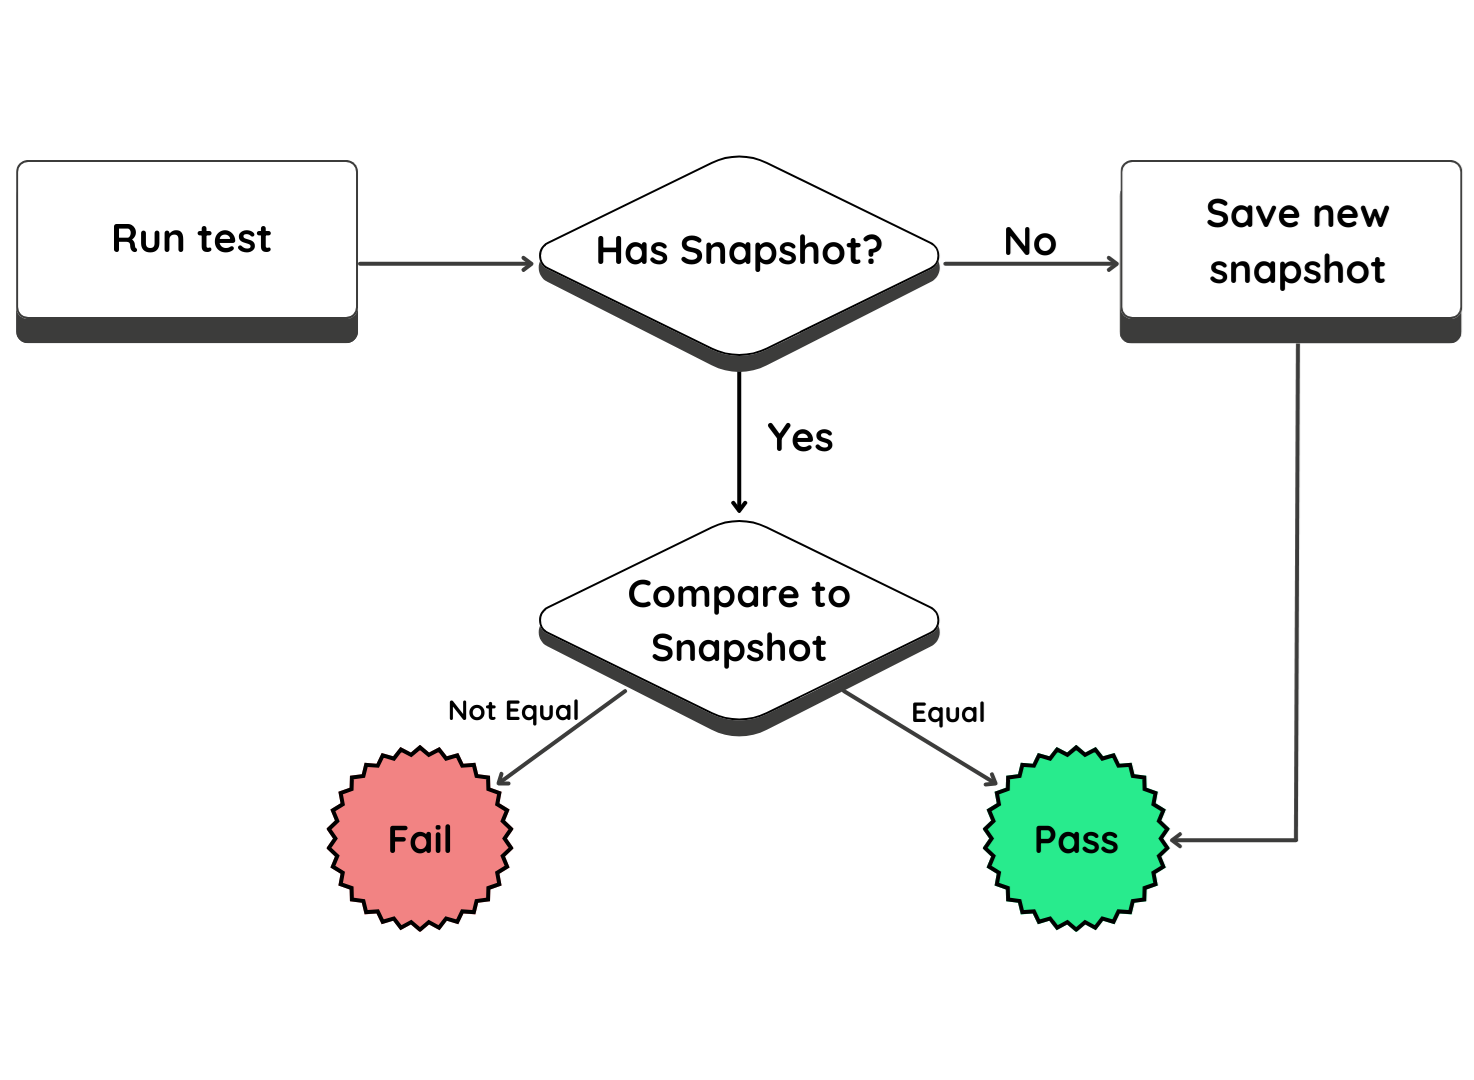
\includegraphics[width=0.75\textwidth]{img/snapshot-test-workflow-2.png}
            \caption{Snapshot testing workflow.}
            \label{fig:snapshot-test-workflow}
        \end{figure}

    When a snapshot test fails, the testing framework highlights and displays the differences between the snapshot and the current state. There are two possible causes for such differences:
        
    \begin{itemize}
        \item The differences are indeed a consequence of a bug introduced in the code (true positive).
        \item The difference is caused by an intended change in the code, for example, to support a new requirement or a changing one (false positive).
    \end{itemize}

    When a false positive happens, developers should update the snapshot, introducing a new golden standard based on the current state, and thus resolving the failed test.\\
    
    Testing frameworks such as Jest have the option of encoding snapshots into a file, making it simpler to check the tests on further runs, and also working as an artifact to be reviewed as part of a code review process~\cite{Jest22}. When it comes to identifying unwanted modifications in user-facing components, serialized data, and other complex objects, this technique has shown to be particularly beneficial~\cite{osmani2018}.

    The roots of snapshot testing can be traced back to broader testing practices outlined in Feathers’ work on software maintenance, particularly in his discussion of characterization testing~\cite{feathers2004legacy}. Feathers introduces characterization testing as a strategy for understanding and preserving existing system behavior when making code modifications, especially in legacy systems. This approach emphasizes creating tests that characterize the current behavior of a system, allowing developers to detect unintended changes without needing complete knowledge of the underlying code~\cite{feathers2004legacy}. Snapshot testing builds on this principle by capturing a snapshot of a component’s output, aligning with the goals of characterization testing, and helping developers confidently refactor or enhance code by providing a reliable mechanism to catch regressions. Snapshot testing may not be just a tool for detecting regressions but part of a broader framework that helps safeguard and understand system behavior during development.

    \section{Jest}\label{sec:ch2-jest}

    Jest is widely regarded by software developers as a robust and reliable testing framework. It currently has over 21 million weekly downloads and 43,000+ GitHub stars, making it the most used testing framework for JavaScript and TypeScript. It is used by many companies including Amazon, Google, Microsoft, and Stripe, among others~\cite{OpenJS2024}. Initially developed by Meta, Jest became popular and is now part of the OpenJS Foundation, which supports collaborative development of JavaScript and web technologies. Its ease of use and versatility make it a popular tool for automating tests in various contexts, including unit, integration, and end-to-end testing.
    From frontend web development to more extensive backend logic, Jest's features enable developers to build, run, and analyze tests effectively, therefore offering a complete set of testing capabilities and supporting a range of applications~\cite{Jest22}. Moreover, Jest easily connects with popular libraries and frameworks like React\footnote{\url{https://www.react.dev/}} and Node.js\footnote{\url{https://www.nodejs.org/en}}, increasing its popularity throughout many projects. With an active open-source community, Jest keeps changing to match contemporary development practices and confirms its importance as a necessary tool to help preserving JavaScript or TypeScript application's software quality.

    In addition to its support for various testing types, Jest also incorporates snapshot testing, considered to be valuable for checking the structure and output of components' state and other serialized data. Writing a snapshot test in Jest is straightforward, involving only a few lines of code.
    
    Suppose we are using React to develop a web component to display a small icon for a social media link.\footnote{This example is inspired by the snapshot test example in the Jest webpage: \url{https://www.jestjs.io/docs/snapshot-testing/}} Initially, the only social media we have is Facebook and we hard coded it into our React component (Listing~\ref{lst:snapshot-test-example-social-media-icon}). In this component, we have a link (line 4) with the Facebook logo (line 5). Figure 2 shows the expected display for that component.

    \begin{lstlisting}[language=javascript, caption= \texttt{SocialMediaIcon} React component, label=lst:snapshot-test-example-social-media-icon]
// SocialMediaIcon.js
export default function SocialMediaIcon() {
    return(
        <a href="http://www.facebook.com">
            <i className='bi bi-facebook'></i>
        </a>
    );
}
    \end{lstlisting}

    \begin{figure}[h]
        \centering
        
\includegraphics[width=96px]{exemplo/img/facebook-logo.png}
        \caption{Facebook logo icon.}
        \label{fig:facebook-logo}
    \end{figure}

    React makes it possible to reuse our components in other parts of a project. Listing~\ref{lst:snapshot-test-example-main-footer} shows an example of using \texttt{SocialMediaIcon} in another component called \texttt{MainFooter}.

    \begin{lstlisting}[language=javascript, caption= (Re)using \texttt{SocialMediaIcon} in another component, label=lst:snapshot-test-example-main-footer]
// MainFooter.js
import SocialMediaIcon from './SocialMediaIcon';

export default function MainFooter() {
    return(
        <div>
            <SocialMediaIcon />
            {/* This component can contain other footer components */}
        </div>
    );
}
    \end{lstlisting}

    To guarantee that our component does not change without our knowledge, we create a snapshot test for it, as shown in Listing~\ref{lst:snapshot-test-example-jest}.

    \begin{lstlisting}[language=javascript, caption= Snapshot test example for a \texttt{MainFooter} component, label=lst:snapshot-test-example-jest]
// MainFooter.spec.js
import TestRenderer from 'react-test-renderer';
import MainFooter  from './MainFooter';

test('MainFooter renders correctly', () => {
     const tree = TestRenderer
        .create(<MainFooter/>)
        .toJSON();
     expect(tree).toMatchSnapshot();
});
    \end{lstlisting} 

In this listing, the code demonstrates a basic snapshot test for a React \texttt{MainFooter} component using the Jest testing framework. First, in line 2, we import the \texttt{TestRenderer} module from the \texttt{react-test-renderer} library, which provides a \texttt{TestRenderer} that can be used to render React components to pure JavaScript objects, without depending on the DOM. Essentially, this package allows the serialization of a component into a in-memory tree so that the developer can make test assertions about it later.\footnote{\url{https://www.legacy.reactjs.org/docs/test-renderer.html\#overview}} Following this, line 3 imports the \texttt{MainFooter} component from the project’s structure \texttt{('./MainFooter')}. The test function itself is defined in line 5 with \texttt{test ('MainFooter renders correctly', () =$>$ \{...\});}, where the phrase ``MainFooter renders correctly" is a descriptive label indicating the expected behavior of the test.

Moving to line 6, we declare the constant \texttt{tree}, which will hold the object representing the rendered tree of the component. Then, \texttt{TestRenderer.create(...)} is invoked in line 7 to create a \texttt{TestRenderer} instance with the passed \texttt{MainFooter} element, for it to be rendered and to mount its view hierarchy (similar to a HTML DOM tree), thus giving developers a readable structure of what the output would look like in the browser. Later, in line 8, the \texttt{toJSON()} method is called, returning an object representing this rendered tree, containing only the native nodes, in this case \texttt{<div>}, \texttt{<a>}, \texttt{<i>} and their properties.\footnote{\url{https://legacy.reactjs.org/docs/test-renderer.html\#testrenderertojson}} This serialization allows Jest to compare or create the current state in a stored snapshot in line 9, where the test asserts that the generated representation (\texttt{tree}) matches the stored snapshot with \texttt{expect(tree).toMatchSnapshot()}.

When this test runs for the first time, Jest creates a snapshot file as demonstrated in Listing ~\ref{lst:snapshot-test-example-file}.

    \begin{lstlisting}[language=javascript, caption= Snapshot file example for a \texttt{MainFooter} component, label=lst:snapshot-test-example-file]
// __snapshots__/MainFooter.spec.js.snap
//Jest Snapshot v1, https://goo.gl/fbAQLP

exports[`MainFooter renders correctly 1`] = `
<div>
  <a
    href="http://www.facebook.com"
  >
    <i
      className="bi bi-facebook"
    />
  </a>
</div>
`;
    \end{lstlisting} 


From then on, this test checks if the rendered component matches the previously saved snapshot. If they differ, Jest will report a failure, indicating a change in the component's output, which could be intentional or due to an error.

Suppose, for example, that some days later, another developer adds another social media link besides Facebook. Particularly, the developer changes the \texttt{SocialMediaIcon} component to receive the name as property (Listing~\ref{lst:snapshot-test-example-social-media-icon-2}).

    \begin{lstlisting}[language=javascript, caption= Refactored \texttt{SocialMediaIcon} component, label=lst:snapshot-test-example-social-media-icon-2]
// SocialMediaIcon.js
export default function SocialMediaIcon(props) {
    return(
        <a href={`http://www.${props.name}.com`}>
            <i className={`bi bi-${props.name}`}></i>
        </a>
    );
}
    \end{lstlisting}


Now to properly use the modified component, one must call \texttt{<SocialMediaIcon name="facebook" />}. However, suppose the developer forgets to update the \texttt{MainFooter} component, which will therefore invoke the \texttt{SocialMediaIcon} component without the name property. In JavaScript, by omitting a property, its value becomes undefined. After implementing the change, the developer runs the test suite. The snapshot test (Listing~\ref{lst:snapshot-test-example-jest}) will fail and Jest will produce a diff result as the one in Figure~\ref{fig:snapshot-diff}. This warns the developer that he/she forgot to update one of the pages, and the developer can now fix the issue. 


    \begin{figure}[h]
        \centering
        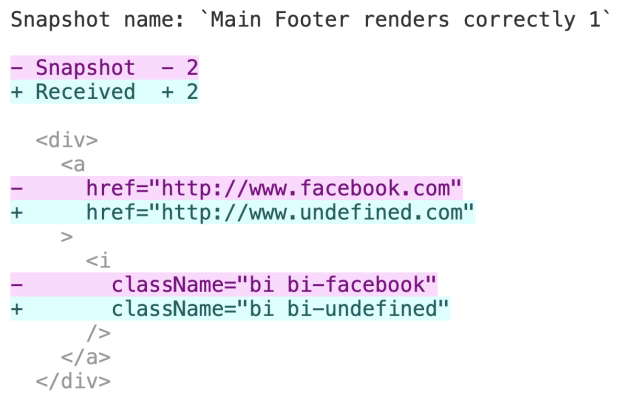
\includegraphics[width=0.75\textwidth]{img/snapshot-diff.png}
        \caption{Snapshot testing difference comparison example.}
        \label{fig:snapshot-diff}
    \end{figure}


With its minimal setup and clear syntax, Jest’s snapshot testing has become a valuable approach for maintaining code consistency and ensuring user interface and user experience stability across versions~\cite{Fontana2015}. Newer versions of Jest's snapshot testing framework also provide auxiliary assertion types to capture and compare error messages thrown, facilitating testing consistent error handling throughout the application's lifecycle~\cite{bekkhus2017jest22}. As highlighted in the documentation, this feature simplifies the validation of error outputs, aiding in tracking changes to error handling and expediting debugging.
    
While snapshot testing in Jest offers an interesting mechanism for maintaining consistency, it is not without its challenges. Over time, snapshot tests as well as other types of tests can become difficult to manage, especially as applications grow and evolve, leading to issues commonly referred to as test smells, which we will discuss next.  

    \section{Test Smells}\label{sec:ch2-test-smells}

    Test smells are indicators of potential flaws in test code that can make tests more difficult to maintain, less reliable, or more likely to fail. Similar to code smells that are associated with code in general programming, test smells frequently come out as the result of bad design choices, a lack of clarity, or inefficient practices when writing automated tests~\cite{Fowler2018}. The presence of test smells may result in tests that are not easy to comprehend, that are susceptible to alterations, or that produce results that are not clear. It is possible that these issues can hinder the detection of actual defects, which will influence software assurance~\cite{beck2003}. Recognizing these test smells is essential for writing clean, efficient, and reliable tests, ensuring the long-term health of a test suite.

    Refactoring is a process of restructuring existing code without altering its external behavior to improve its internal structure and readability. It is a technique widely adopted to mitigate test smells. It involves cleaning up code, simplifying complex logic, and removing redundancies to make the codebase more efficient and easier to work with. Best practices for eliminating test smells, for example, include breaking down large tests into smaller, more focused ones, avoiding complex logic in tests, and ensuring that the tests are easily comprehensible~\cite{Fowler2018}.

    Developers should familiarize themselves with the extensive catalog of test smells that can compromise the effectiveness of automated testing and overall software quality. Notable among these are overly large tests, which can become cumbersome and difficult to maintain, and tests with conditional logic, which introduce unnecessary complexity into test cases~\cite{beck2003}. The following sections will introduce these two issues, exploring their characteristics and highlighting the problems they cause.
    
    \subsection{Large Test}\label{sec:ch2-test-smells-large-test}

    A large test smell occurs when an automated test case becomes excessively large, complex, or unwieldy. Such tests are typically difficult to understand, maintain, and debug, as their scope extends beyond a single, well-defined behavior or unit~\cite{Osherove2009}. They might involve numerous dependencies, complex setups, or extensive configurations that make them prone to errors and instability. Large test smells can lead to slower test execution times and increase the likelihood of false positives and negatives, ultimately diminishing the effectiveness of the testing process~\cite{Meszaros2007}. By violating principles of simplicity and modularity, large tests also hinder a clear assessment of code functionality and obscure the root cause of failures, complicating the development and maintenance of test suites~\cite{Fontana2015}. Listing~\ref{lst:large-test-smell-example} presents an example of a large test in JavaScript.\\

        \begin{lstlisting}[language=javascript, caption= Large test smell example, label=lst:large-test-smell-example]
// calculator.test.js
const Calculator = require('./calculator');
const calculator = new Calculator();

test('Calculator performs various operations correctly', () => {
    // Test addition
    expect(calculator.add(2, 3)).toBe(5);
    expect(calculator.add(-2, -3)).toBe(-5);
    expect(calculator.add(2, -3)).toBe(-1);
    // Test subtraction
    expect(calculator.subtract(5, 3)).toBe(2);
    expect(calculator.subtract(3, 5)).toBe(-2);
    // Test multiplication
    expect(calculator.multiply(2, 3)).toBe(6);
    expect(calculator.multiply(-2, 3)).toBe(-6);
    expect(calculator.multiply(0, 5)).toBe(0);
    // Test division
    expect(calculator.divide(6, 3)).toBe(2);
    expect(calculator.divide(5, 2)).toBe(2.5);
    expect(() => calculator.divide(5, 0)).toThrow('Cannot divide by zero');
    // Test power
    expect(calculator.power(2, 3)).toBe(8);
    expect(calculator.power(5, 0)).toBe(1);
    // Further calculator testing scenarios...
});
        \end{lstlisting}
        ~\\[-2.0pt]

        Lack of organization and concentration in this test code produces a large test smell, therefore compromising test maintainability and clarity. Violating the single-responsibility principle, this test aggregates several unrelated operations—addition, subtraction, multiplication, etc.—into a single test case. Since the entire test is combined, it can be difficult to identify the particular activity or scenario generating a problem when something fails.
    
        \subsection{Test with Conditional Logic}\label{sec:ch2-test-smells-conditional-logic}

        This test smell arises when a test case includes conditional statements, such as \texttt{if}, \texttt{else}, \texttt{switch}, or loops that vary the test’s behavior based on different scenarios or data conditions. This smell indicates the test is verifying multiple paths or behaviors within a single test case, leading to increased complexity and reduced readability. Conditional logic within tests is problematic because it complicates understanding what specific behavior is being verified, making it harder to diagnose failures and maintain the test~\cite{beck2003,Meszaros2007,Valente24}. Listing~\ref{lst:conditional-logic-test-smell-example} presents an example of a conditional logic test in JavaScript.\\

                \begin{lstlisting}[language=javascript, caption= Conditional logic test smell example, label=lst:conditional-logic-test-smell-example]
 // userValidator.test.js
 const UserValidator = require('./userValidator');
 const validator = new UserValidator();

 test('UserValidator correctly validates users', () => {
     const users = [
         { age: 20, country: 'US' },
         { age: 17, country: 'US' },
         { age: 25, country: 'CA' },
         { age: 30, country: 'UK' },
     ];
     users.forEach((user) => {
         let expected;
         if (user.age >= 18) {
             if (user.country === 'US' || user.country === 'CA') {
                 expected = true;
             } else {
                 expected = false;
             }
         } else {
             expected = false;
         }
         expect(validator.isValidUser(user)).toBe(expected);
     });
 });
         \end{lstlisting} 

         This test code suffers from a conditional logic smell because of the nested \texttt{if} and \texttt{else} statements, which increase the complexity of the test. These nested conditions impede quick understanding of the expected results for every input, in this case validating users age and country, therefore compromising the test's maintainability and readability. Simple, declarative tests should clearly define the inputs and expected results without adding needless levels of logic.

    \section{Continuous Integration and Delivery}\label{sec:ch2-ci}

    Continuous Integration (CI) is an approach for software development in which developers integrate code into a shared repository on multiple occasions throughout their development schedule. In it, the application is built, and then a series of automated tests are executed against it. Then, each time a new commit is added to the codebase, this process is repeated~\cite{Bass2015}. This practice was popularized by Fowler~\cite{fowler2006ci}, who highlighted the importance in reducing integration problems and enhancing software quality in a fixed schedule.

    Continuous Delivery (CD) is another approach in which teams produce software in short cycles, ensuring that the software can be reliably released at any time~\cite{humble2010}. It builds upon Continuous Integration by automating the release process, so that deployments can be performed quickly, sustainably, and on demand. The goal of this practice is to make software delivery more efficient and less risky by reducing the time between code integration and actual deployment~\cite{Bass2015}.

    When combined, these two practices create a seamless workflow that allows development teams to deliver software more efficiently and reliably. CI ensures that code changes are regularly integrated and tested, while CD automates the release process, making sure that those changes can be deployed to production at any time~\cite{Bass2015}. The adoption of these practices can provide benefits such as faster time-to-market, improved software quality, reduced deployment risks, enhanced team collaboration, and increased customer satisfaction due to more frequent and reliable software releases~\cite{crispin2009}. Figure~\ref{fig:ci-cd-workflow} summarizes the CI/CD workflow.\\

    \begin{figure}[h]
        \centering
        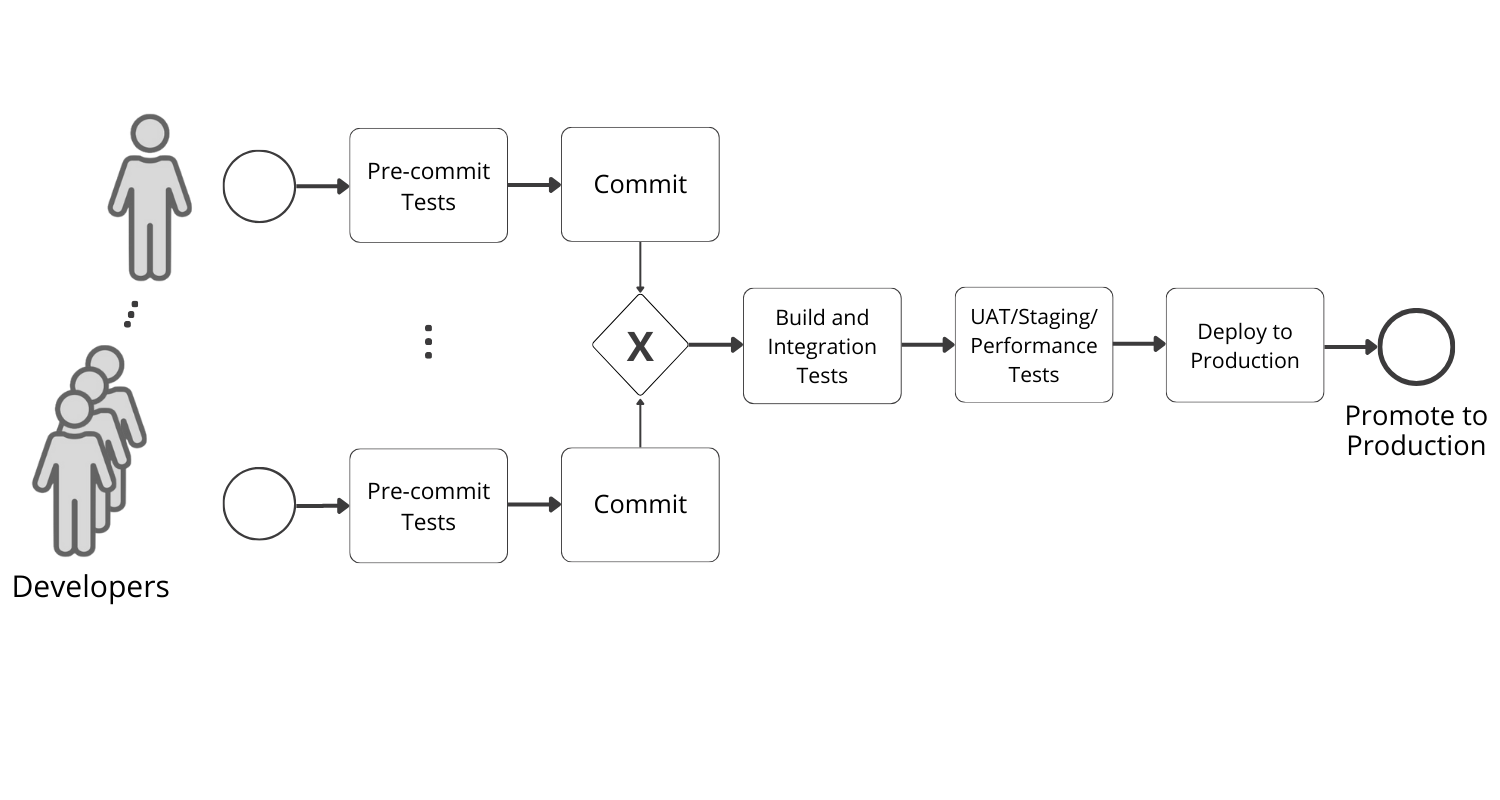
\includegraphics[width=\textwidth]{img/cicd.png}
        \caption{Continuous Integration and Continuous Delivery pipeline workflow.}
        \label{fig:ci-cd-workflow}
    \end{figure}

    \subsection{GitHub Actions}\label{sec:ch2-github-actions}

        GitHub Actions provides a means for implementing continuous integration and continuous delivery (CI/CD) in open-source projects hosted on GitHub, enabling developers to automate tasks like testing, building, and deploying applications whenever changes are made to a repository~\cite{GitHub_CI}.

        The execution of automated tests in continuous integration pipelines is a typical use for GitHub Actions. GitHub Actions guarantees automated tests are automatically executed as part of the development cycle by allowing users to build up processes that trigger on events such as pull requests or commits. Through the use of this integration, teams may detect regressions at an earlier stage and preserve the integrity of their codebases across upgrades~\cite{GitHub_Actions}. An example of a workflow that is written in YAML and is part of the continuous integration process is presented in Listing~\ref{lst:example-wkflow}.

        \begin{lstlisting}[language=yaml, caption=GitHub Actions workflow example, label=lst:example-wkflow]
name: CI/CD Pipeline
run-name: Build, Test, and Deploy on Push
on:
  push:
    branches:
      - main
jobs:
  test-build-and-deploy:
    runs-on: ubuntu-latest
    steps:
      - name: Check out repository code
        uses: actions/checkout@v4
      - name: Set up Node.js
        uses: actions/setup-node@v3
        with:
          node-version: '18'  
      - name: Install dependencies
        run: npm install
      - name: Run tests
        run: npm test
      - name: Build project
        run: npm build
      - name: Deploy project
        run: npm run-script deploy
\end{lstlisting} 
~\\[-2.0pt]

The provided code is a configuration file for a pipeline that automates testing, building, and deploying a Node.js application. In line 1, we define a name for the pipeline. In line 2, we define the name for a given run. In lines 3-6, we define that this pipeline will be triggered automatically whenever there is a push event to the main branch. In lines 7-26, we define the \texttt{test-build-and-deploy} job created by the developer, which contains the tasks to be executed in the pipeline. This job is configured to run on the \texttt{ubuntu-latest} environment, as specified in line 9, using a virtual Ubuntu machine. In line 10, we start describing a series of steps.

In line 11, the first step, named check out repository code, uses the \texttt{actions/check\-out@v4} action (line 12) to clone the repository code into the execution environment, ensuring that subsequent steps can access the necessary files. In line 13, we set up Node.js using \texttt{actions/set\-up-node@v3} action (line 14) and specify version 18 (lines 15-16), which will be used for all subsequent steps in the pipeline. In line 17, we install the project dependencies using the command \texttt{npm install} (line 18), preparing the environment for testing and building. Next, in line 19, the Run tests step runs \texttt{npm test} (line 20), where the pipeline executes the project’s test suite to ensure that the pushed code works as expected and does not introduce any failures. In line 21, the Build project step runs the \texttt{npm build} command (line 22), which compiles the project and generates the code ready for deployment. Finally, in line 23, the Deploy project step runs the \texttt{npm run-script deploy} command (line 24) to deploy the project, allowing the latest version of the code on main branch to be available for production. 

    \section{Grey Literature}\label{sec:ch2-grey-literature}

        Grey literature refers to information produced on all levels of government, academia, business, and industry that is not controlled by commercial publishers. This includes documents like technical reports, white papers, theses, conference proceedings, and government publications~\cite{Farace2010}. Unlike traditional academic literature, grey literature is often disseminated through informal channels and may not undergo rigorous peer review. The term ``grey" highlights its status as information that falls outside the conventional academic publishing spectrum, making it less visible and harder to access but nonetheless valuable~\cite{Weintraub2000, Lawrence2015}.

        A grey literature review is a process that involves searching for, evaluating, and synthesizing information from grey literature sources in a methodical manner~\cite{Adams2017}. Traditional literature evaluations are complemented by these reviews, which capture a wider variety of information. This includes the most recent discoveries and practical insights, which may not yet be represented in journals that are subject to peer review~\cite{Paez2017}. Due to concerns such as a lack of consistency, varying quality, and challenges in obtaining and accessing information, doing a grey literature review can be a complex and risky endeavor. However, the incorporation of grey literature not only enriches the evidence base but also provides a more comprehensive grasp of the subject matter of a research project~\cite{Farace2010}.

        Due to the fast rate at which technology advances, grey literature is of utmost significance in the field of software engineering. The documentation of several novel methods, tools, and methodologies can be found in white papers, technical reports, or even software developers blogs~\cite{Garousi2019}. This documentation occurs well in advance of their publication in academic journals. By incorporating grey literature into reviews, software engineers and researchers can gain access to the most recent information, acquire insights into the patterns that are occurring in the industry and bridge the gap between theory and practice~\cite{Garousi2016}. Not only does this improve the relevance of research, but it also contributes to improved decision-making in software development initiatives. Researchers, for example, often consult sources of grey literature in order to study novel approaches to what has not been studied yet~\cite{Adams2017, Vegi2022, Vegi2023, Gazzinelli2023JSS}.

        \section{Test Pyramid}\label{sec:ch2-test-pyramid}

        \begin{figure}[h]
            \centering
            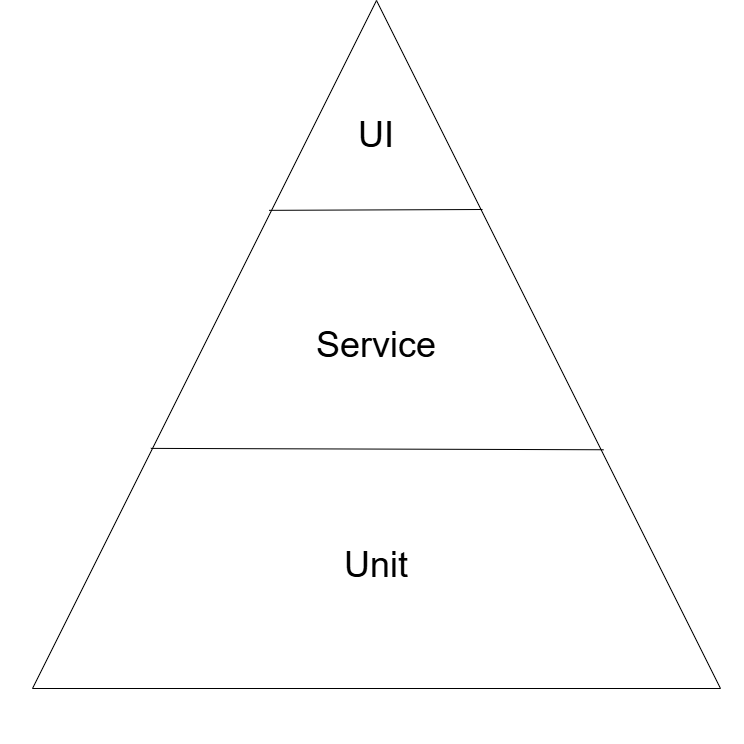
\includegraphics[scale=0.45]{img/test_pyramid.png}
            \caption{Software testing pyramid}\label{fig:test_pyramid}
        \end{figure}

        The Test Pyramid, introduced by Mike Cohn~\cite{Cohn09}, is a conceptual model that helps software teams structure their test suites efficiently. It advocates a balanced testing strategy by emphasizing a higher number of low-level unit tests, a moderate number of integration tests, and fewer high-cost UI or end-to-end (E2E) tests. This structure aims to optimize test execution time, improve feedback loops, and enhance maintainability while minimizing reliance on brittle UI tests, represented as a three-layered structure:

        \begin{itemize}
        
            \item\textbf{Unit Tests (Base Layer):} These tests form the foundation of the pyramid and validate individual components in isolation. They are fast, reliable, and cost-effective, making them the preferred choice for regression detection.
            
            \item\textbf{Integration Tests (Middle Layer):} These tests assess the interaction between modules, ensuring that components work together as expected. They are slower than unit tests but critical for detecting issues in system interactions.
            
            \item\textbf{End-to-End (E2E) Tests (Top Layer):} These tests simulate real user workflows, verifying that the entire system functions as intended. However, they are costly in terms of execution time and maintenance, making it impractical to rely on them extensively.
            
        \end{itemize}
        

        \section{Related Work}\label{sec:ch2-related-work}

        Snapshot testing has gained attention as an effective testing approach, primarily within the industry. However, the technique is relatively new and lacks extensive academic research, with very few studies dedicated to understanding its practices and adoptions in open-source projects. This section reviews not only existing literature on snapshot testing but also highlights other studies within the broader context of this software testing approach and its methods.
        
        Fujita et al.~\cite{fujita2023empirical} extended the understanding of snapshot testing through an empirical study focused on the adoption of snapshot testing across various open-source projects using the Jest framework. Their research examined the evolution of snapshot testing over time, revealing common patterns of adoption and co-evolution with other types of tests, such as unit tests. Their analysis found that repositories implementing both snapshot and unit tests tended to have a more substantial number of test cases, suggesting a complementary role for snapshot testing alongside more traditional test types. Additionally, the authors identified frequent updates to snapshot files as part of development workflow, underscoring the technique's adaptability to evolving software but also hinting at the need for more rigorous management practices to avoid misalignment between snapshots and current versions.

        Goldberg~\cite{goldberg2023best} suggests a standardization approach to snapshot testing, advocating for the use of inline snapshots only when necessary and keeping them concise, emphasizing that shorter, more targeted snapshots allow for clearer and more maintainable tests.

        Other research within software testing provides indirect insights into snapshot testing practices. For instance, work on automated UI testing tools, like those by Borjesson and Feldt~\cite{Borjesson2012}, discusses similar challenges in automated testing, such as tool fragility and the difficulties inherent in regression testing for visual components. End-to-end (E2E) testing, which verifies the complete functionality of an application by simulating user interactions, shares some conceptual similarities with snapshot testing in ensuring UI consistency and detecting unintended changes. Studies on end-to-end testing frameworks, such as Selenium, Cypress, and Playwright, highlight challenges related to test flakiness, environment dependencies, and the high maintenance costs of UI-based tests~\cite{Stocco2018}. These challenges align with issues observed in snapshot testing, such as test brittleness and unintended failures due to minor UI modifications. Moreover, broader discussions in software testing research emphasize the need for balancing automated verification with human oversight, particularly when dealing with visual or structural changes in application interfaces~\cite{Garousi2020}. 
        
        Studies examining test smells, as conducted by Tufano et al.~\cite{tufano2016test}, also offer a relevant lens, particularly regarding certain test smells, such as large, unreadable tests or unstructured, non-linear test logic, which can decrease test maintainability. Additionally, studies focused on JavaScript testing, such as those by Mirshokraie et al.~\cite{mirshokraie2015jseft}, explore testing complexities in the dynamic language environment of JavaScript. These studies, while not directly addressing snapshot testing, provide broader perspectives on automated regression testing challenges, offering valuable comparisons and frameworks for interpreting the limitations and practical applications of testing techniques. Another study, by Rafique et al.~\cite{Rafique2012}, explores testing patterns in open-source projects, noting that regression testing practices vary significantly based on the language and framework. Additionally, the authors also highlight that regression testing is important in maintaining reliability, particularly as CI/CD pipelines introduce automation to development workflows.

        Research in the field of software engineering has demonstrated that idioms, which are low-level patterns of recurring syntactic fragments with a single semantic role, can be effectively mined from source code and common assertions~\cite{buschmann1996patterns}. The work of Allamanis and Sutton~\cite{allamanis2014mining} introduced a framework to automatically identify code idioms from large corpora of idiomatic software projects.
        
        

    \section{Final Remarks}\label{sec:ch2-final-remarks}
    
        In this chapter, we covered key concepts in software assurance and testing, snapshot testing, the Jest framework, and common test smells. We also explored continuous integration, continuous deployment and the GitHub Actions tool for continuous integration pipelines and the importance of grey literature reviews in software engineering.

        In the chapters that follow, we report two studies on snapshot testing, one is a grey literature review to identify benefits, drawbacks, best practices, commonly tested components, and testing frameworks associated with snapshot testing. The other is an empirical study on snapshot testing practices with Jest, where we uncover its key characteristics, common patterns, less-common cases, and refactoring suggestions for these tests as identified in open-source repositories. Additionally, we investigate the potential inclusion of snapshot tests as part of continuous integration and continuous delivery pipelines. The background information presented in this section provides essential context for understanding the aspects explored in such studies.

     \chapter{Grey Literature Review}

        In this chapter, we perform a grey literature review in order to understand and characterize the state of snapshot testing in the software development community. Our goal with this study is to identify and analyze the main benefits, drawbacks, best practices, commonly tested components, and testing frameworks associated with snapshot testing, as described by practitioners. Section~\ref{sec:ch3-intro} makes a brief introduction to our grey literature review. Section~\ref{sec:ch3-rqs} defines our research questions. The design of our study is detailed in Section~\ref{sec:ch3-study-design}. Section~\ref{sec:ch3-results} presents the results obtained in this review. Section~\ref{sec:ch3-key-findings} highlights the key contributions of this research. The discussion of our findings is presented at Section~\ref{sec:ch3-discussion}. Threats to validity are discussed in Section~\ref{sec:ch3-threats}. Finally, Section~\ref{sec:ch3-final-remarks} concludes the chapter.

        \section{Introduction}\label{sec:ch3-intro}

        For our review, we gathered and labeled fifty documents, which included blog posts, forum discussions, and video transcripts. Moreover, these documents were only collected from authors who had at least two years of experience in software development, reputable blogs, official documentation, and well-known forums. Our objective was to collect information regarding the advantages, disadvantages, and best practices of adopting snapshot testing. We also investigated how common snapshot testing is when it comes to testing frameworks and architectural components. By addressing these aspects, this study seeks to offer insights into the tradeoffs involved in snapshot testing, providing information to help developers make informed decisions about its use and implementation in software projects.

        \section{Research Questions}\label{sec:ch3-rqs}

        We elaborated the following research questions to guide the information collection for our grey literature review:\\

        \begin{itemize}
          \item \textbf{RQ3.1: What are the main benefits of snapshot tests?}
            Our objective with this question is to provide an examination of the specific benefits that developers describe in relation to this practice.
         \item \textbf{RQ3.2: What are the main drawbacks of snapshot tests?} 
            Developers have reported drawbacks when adopting Snapshot testing that should be considered.
         \item \textbf{RQ3.3: What are the best practices when using snapshot tests?}
            Addressing some of the drawbacks found in the previous RQ, we investigate recommended practices in order to facilitate maintenance and lead to an easier understanding of snapshot tests.
            \item \textbf{RQ3.4: What architectural components are tested using snapshot testing?}
            Snapshot testing is relevant to an extensive range of architectural components in a software system. Therefore, we evaluate the major architectures in which developers utilize this practice.
            \item \textbf{RQ3.5: Which libraries and tools are commonly used for implementing snapshot tests?}
            Snapshot testing is currently supported by numerous libraries and testing frameworks. Our aim is to enumerate the tools often utilized by developers.
        \end{itemize}
     
		\section{Study Design}\label{sec:ch3-study-design}

        We conducted a grey literature review to address the five research questions mentioned. Our goal was to better understand Snapshot Testing according to practitioners. Grey literature has shown as a reliable source for this novel technique~\cite{kamei2021information}. The method used for this investigation consisted of a few steps, which are shown in Figure~\ref{fig:grey-literature-design-study}. In this method, one hundred documents were gathered for snapshot testing, and then a series of filters were used to choose the top fifty for further in-depth examination, analysis, and validation. We split our work into five steps:

        \begin{figure}[h]
            \centering
            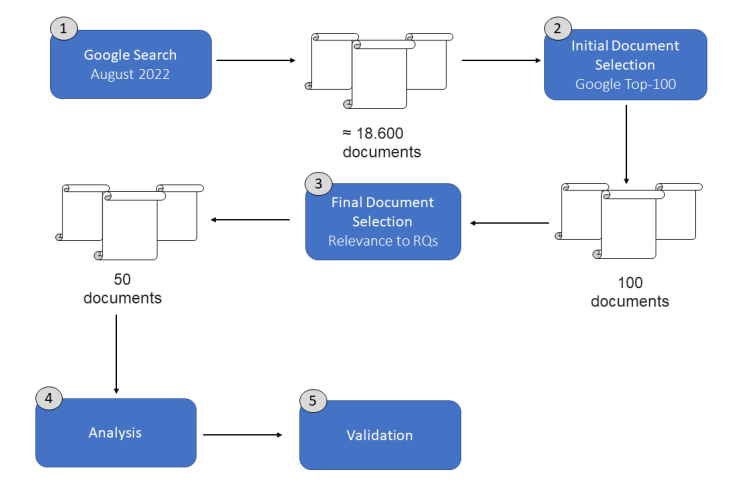
\includegraphics[width=\textwidth]{img/grey_literature_study_design.png}
            \caption{Overview of the grey literature review steps.}\label{fig:grey-literature-design-study}
        \end{figure}

        \begin{enumerate}

            \item \textbf{Google Search:} Before executing a search for documents on Google, it is important to calibrate the query strings (for instance, by combining synonyms or removing terms that may impact the results). After conducting this calibration, we decided to use the following query: ("snapshot testing") AND ("benefits" OR "limitations").

            \item \textbf{Initial Document Selection}: Since about 18,600 documents were retrieved by the search, a full review of them would be impracticable. Therefore, and as is common in grey literature reviews~\cite{kamei2021information}, it is necessary to restrict the number of articles subjected to in-depth reading and analysis. Thus, we concentrate on the first ten pages of search results, i.e., the top 100 documents returned by Google search.

            \item \textbf{Final Document Selection:} We read these 100 documents to identify and retain only those relevant to the proposed RQs. In the end, we selected 50 documents for analysis, which we refer to as D1 to D50. All selected documents originate from rather credible sources. Specifically, most of the included materials were authored by individuals with at least two years of professional software development experience (verified via LinkedIn). Additionally, we also considered content from well-established technical blogs known in the industry (e.g., The Software House), from the official documentation of testing frameworks (such as Jest) and from active developer forums with substantial community engagement (e.g., Stack Overflow and GitHub Discussions). Table~\ref{tab:source_documents} shows the distribution of documents among these categories. A single source was attributed to each document (the first source that applies, following the order they are listed in the table). For this reason, the sum of the percentages is 100\%.
            
            \hspace{1pt}
            \begin{table}[!ht]
            \centering
            \begin{tabular}{p{5cm}S[table-format=2]S[table-format=2]}
                \toprule
                \textbf{Source} & {\textbf{Documents (\%)}} & {\textbf{Documents (Freq)}} \\
                \midrule
                Reputable Author       & 76\% & 38 \\
                Reputable Blog         & 10\% & 5  \\
                Official Documentation & 8\%  & 4  \\
                Forum Discussion       & 6\%  & 3  \\
                \bottomrule
            \end{tabular}
            \caption{Source of the selected documents.}
            \label{tab:source_documents}
            \end{table}
            

            \item \textbf{Analysis:} The documents selected in the previous step were analyzed to answer the proposed research questions. Essentially, we read each document in detail and whenever we found a discussion about benefits (RQ3.1), drawbacks (RQ3.2), best practices (RQ3.3), architectural components (RQ3.4), or tools (RQ3.5) we created a label to denote this discussion (or reused a previously created one) and applied it to the document under analysis. For example, documents commenting on how easy it is to implement snapshot tests received an "Easy to implement" label, which was used to answer RQ3.1. It is important to note that not all selected documents were relevant to every research question. While some documents addressed multiple aspects of snapshot testing, others were focused on a single topic.

            \item \textbf{Validation:} The labels proposed were revised in a cross-validation process between the main author and an advisor. Basically, for each research question, we checked whether the documents associated with each label indeed discuss the label’s theme. In total, we agreed with 224 classifications but also proposed associating 28 labels to documents and removing 34 labels from documents. 
        
        \end{enumerate}

        \noindent In summary, our study design applied a common grey literature review methodology to explore the adoption, benefits, drawbacks, best practices, and tool support of snapshot testing. By leveraging a diverse range of practitioner-authored sources and following a structured process of document selection, analysis, and validation, we ensured a comprehensive view of the state of snapshot testing in practice. This approach allowed us to capture insights from experienced developers and recognized resources, providing a reliable basis for answering our research questions and establishing a foundation for future studies. The following sections present our detailed results across the five research questions.

        \section{Results}\label{sec:ch3-results}

        \subsection{What are the main benefits of snapshot tests? (RQ3.1)}

        The primary advantages of snapshot tests are outlined in Table~\ref{tab:benefits_snapshot_testing} along with the percentage and absolute number (Freq) of documents. Both the ease of implementation and the prevention of regressions were listed as the most cited advantages of snapshot testing.\\

        \hspace{1pt}
        \begin{table}[!ht]
        \centering
        \begin{tabular}{p{7cm}S[table-format=2]S[table-format=2]}
            \toprule
            \textbf{Description} & {\textbf{Documents (\%)}} & {\textbf{Documents (Freq)}} \\
            \midrule
            Easy to implement             & 54\% & 27 \\
            Prevents regression           & 38\% & 19 \\
            Serializable                  & 18\% & 9  \\
            Alternative to UI tests       & 12\% & 6  \\
            Easier and safer refactorings & 10\% & 5  \\
            \bottomrule
        \end{tabular}
        \caption{Main benefits of snapshot testing.}
        \label{tab:benefits_snapshot_testing}
        \end{table}

        Twenty-seven documents (54\%) highlighted the simplicity of creating snapshot tests, often contrasting it with the more complex design and implementation required for traditional unit tests. Authors emphasized that snapshot tests require a single default assertion about the component's state, saving substantial time and effort compared to writing numerous specific assertions. As noted in D3, \textit{“Snapshots with their simplicity can speed up the creation of unit tests (...) snapshot is a single line in comparison to the traditional method.”}, meaning this simplicity can significantly speed up the creation of automated tests. Nineteen documents (38\%) emphasized the effectiveness of snapshot tests in preventing regressions. This benefit comes from the ability to easily compare current and previous component states stored as a snapshot, making it simple to detect unintended changes as mentioned in D37 \textit{“it’s a really, really easy way to see how your changes are impacting some output”}.

        The next benefit points out that snapshots enable programmers to compare and check any serializable value, as commented in 9 documents (18\%). For example, D40’s author states: \textit{"the format of the snapshot is flexible, it can be inlined into the test as a string or stored as a file— it can be a DOM tree, a JSON blob or even a serialized image"}. This distinguishes them from traditional unit tests, where considerable time and effort are usually required to define the best test inputs and outputs. Our second-to-last benefit, as reported by 6 documents (12\%), regards the use of snapshot testing as a faster alternative to UI or end-to-end tests. According to D33, \textit{“(...) I mostly avoid UI tests as they are too complicated to write and time-consuming to run. Snapshot tests are better for SwiftUI, and very fast”}. Our last benefit, reported in 5 documents (10\%) states that snapshots serve as a great tool for easier and safer refactorings, as it can accurately describe, using the snapshot taken, the structure of the component being rendered or the data structure begin returned by the CUT.

        \subsection{What are the main drawbacks of snapshot tests? (RQ3.2)}\label{sec:ch3-drawbacks}
        %\subsection{Drawbacks of Snapshot Testing (RQ3.2)}\label{sec:ch3-drawbacks}
        
        In Table ~\ref{tab:drawbacks_practices_snapshot_testing}, we present the findings of our investigation regarding the drawbacks of snapshot testing.

        \hspace{1pt}
        \begin{table}[!ht]
        \centering
        \begin{tabular}{p{7cm}S[table-format=2]S[table-format=2]}
            \toprule
            \textbf{Description} & {\textbf{Documents (\%)}} & {\textbf{Documents (Freq)}} \\
            \midrule
            Fragility                     & 28\% & 14 \\
            Lack of Context               & 22\% & 11 \\
            Large snapshots               & 16\%  & 8  \\
            Manual Verification           & 12\%  & 6  \\
            Flaky behaviour               & 6\%   & 3  \\
            \bottomrule
        \end{tabular}
        \caption{Drawbacks of snapshot testing.}
        \label{tab:drawbacks_practices_snapshot_testing}
        \end{table}
        
        Despite its benefits snapshot testing also has drawbacks. The most prominent concern, identified in 14 documents (28\%), is the fragility of snapshot tests, stemming from their dependence on the precise output of the component under test. Any change, even a minor one, can cause the test to fail, potentially leading to false positives depending on the nature of the change. D5 aptly explains this: \textit{“a snapshot just tells you what the component looked like before and what it looks like now. The decision whether you’ve fixed a bug, or introduced one, is entirely on you”}, noting that developers bear the full responsibility for determining whether a snapshot difference represents a genuine bug, or a business intended change. Closely related to fragility is the risk of blindly updating snapshots without careful review. D34 highlighted the ease with which developers can update snapshots without understanding the underlying cause of the failure: \textit{“when tests fail, it is very easy to update the snapshots without fixing the code and understanding the failure reason”}. This practice, which was noted by several authors, can mask regressions and lead to decreasing confidence in the test suite.

        Eleven documents (22\%) discussed the lack of context in writing snapshot tests. Because snapshot tests typically use a single, broad assertion, the error messages can be vague and uninformative, especially for larger components with many elements. This can make it difficult to understand what exactly changed and why, hindering debugging efforts as commented by D6: \textit{“we’ve found that in practice, snapshot tests end up making assertions that aren’t clearly represented in the test output. (...) It’s not immediately clear whether something is actually wrong, especially for developers who are unfamiliar with the component”}. Eight documents (16\%) mentioned the issue of large snapshots, particularly for complex components. Large snapshots can be cumbersome to review and manage, especially during merge conflicts. This increases the cognitive load on developers and can slow down the development process due to the complexity of interpreting the diff result as noted in D3, which mentions \textit{“conflict resolution can be a major hassle — resolving merge conflicts in snapshots is a cumbersome task, especially if the snapshot is considerably large”}. Six documents (12\%) pointed out the need for manual verification of snapshot results, even with automated tools. This process, as described in D29, can be time-consuming and error-prone: \textit{“ (...) the biggest problem with manual verification is that it requires a human in the loop. This slows down the process, and is also potentially error-prone.”}. Finally, three documents (6\%) reported issues with flaky behavior in snapshot tests, primarily due to the presence of non-deterministic data (e.g., random UUIDs and current date or time) causing tests to fail intermittently as mentioned by D14: \textit{“one of the most frequent (issues) were non-deterministic JSON outputs, for example, when generating random UUIDs or datetime data. We were frequently facing intermitting failures”}.

        \subsection{What are the best practices when using snapshot tests? (RQ3.3)}
        Table~\ref{tab:best_practices_snapshot_testing} outlines the best practices developers follow to reduce the downsides of snapshot tests.

        \hspace{1pt}
        \begin{table}[!ht]
        \centering
        \begin{tabular}{p{7cm}cc}
            \toprule
            \textbf{Description} & \textbf{Documents (\%)} & \textbf{Documents (Freq)} \\
            \midrule
            Use snapshot tests during code reviews & 26\% & 13 \\
            Treat snapshot results as code         & 22\% & 11 \\
            Write small snapshots                  & 14\% & 7  \\
            Detailed test descriptions             & 6\%  & 3  \\
            \bottomrule
        \end{tabular}
        \caption{Best practices to reduce downsides of snapshot testing.}
        \label{tab:best_practices_snapshot_testing}
        \end{table}
        
        Many best practices were identified to reduce the drawbacks and improve the effectiveness of snapshot testing. Thirteen documents (26\%) stressed the importance of using snapshots during code reviews. By visually comparing changes in snapshots, reviewers can more easily identify unintended behaviors and consequences of code modifications. D9 highlighted how this practice can improve the thoroughness of code reviews, especially for React components: \textit{“ (...) through this process, our team has become more strict on code reviewing these types of tests. We look at exactly what has changed and why. We tend to write a snapshot test as a catch-all for shared React components”}. Eleven documents (22\%) emphasized the need to treat snapshot results as code. This means committing snapshot files alongside the application code and subjecting them to the same version control practices. As D1 states, this ensures that snapshots are considered an integral part of the test suite: \textit{"(...) all snapshot files should be committed alongside the modules they are covering and their tests. They should be considered part of a test, similar to the value of any other assertion"}. Seven documents (14\%) recommended writing small, focused snapshots to improve readability and maintainability. Smaller snapshots lead to even smaller scopes, making it easier to identify specific changes and understand the reasons for test failures. Lastly, Three documents (6\%) suggested including detailed test descriptions to provide context for the snapshots and clarify the intended behavior of the component under test. This helps reviewers understand the main purpose of the test and the significance of any changes in the snapshot.

        \subsection{What architectural components are tested using snapshot testing? (RQ3.4)}
         Table~\ref{tab:components_snapshot_testing} outlines the architectural components where snapshot tests are commonly used.

        \hspace{1pt}
        \begin{table}[!ht]
        \centering
        \begin{tabular}{p{7cm}S[table-format=2]S[table-format=2]}
            \toprule
            \textbf{Component} & {\textbf{Documents (\%)}} & {\textbf{Documents (Freq)}} \\
            \midrule
            Frontend & 56\% & 28 \\
            Mobile   & 28\% & 14 \\
            Backend  & 8\%  & 4  \\
            \bottomrule
        \end{tabular}
        \caption{Components tested using snapshot tests.}
        \label{tab:components_snapshot_testing}
        \end{table}

        As expected, snapshot tests are mostly used in the frontend (28 documents, 56\%). In fact, as we mentioned in RQ3.1, they are seen as an alternative to traditional UI or end-to-end tests. For example, D15 mentions the following about the test of React-based JavaScript frontends: \textit{“snapshot testing has been created due to the need for an easier way to write tests for React components. Many React developers reported that they spend more time writing tests than the actual component. Therefore, snapshot testing allows React developers to quickly generate tests using its simple syntax”}.

        In addition, snapshot tests also play an important role in mobile development, particularly when it comes to examining how displayed layouts or views behave across a wide variety of different devices and orientations. Among other uses, D13 provides the following description: \textit{“within our test suite, we utilized a well-crafted loop to iterate through all combinations of the five cell parameters, so that we could quickly and exhaustively generate views for all valid combinations for devices sizes and orientations. (...) As the tooling and frameworks mature and experience with this technique grows, snapshot testing will become even more reliable and is already a worthy addition to any large-scale mobile project”}.

        Finally, snapshot testing is less prevalent in the backend (four documents, 8\%). However, in these components, one interesting use case we found is that they can be used to check for warning and error messages, as explained by D28’s author \textit{“(...) it’s a really common case that you want to write a test to ensure that a good error or warning message is logged to the console... Before snapshot testing I would always write a silly regex that got the basic gist of what the message should say, but with snapshot testing it’s so much easier”}.

        \subsection{Which libraries and tools are commonly used for implementing snapshot tests? (RQ3.5)}
         Table~\ref{tab:libraries_snapshot_testing} lists the libraries and tools used to support snapshot tests. 

        \hspace{1pt}
        \begin{table}[!ht]
        \centering
        \begin{tabular}{p{7cm}S[table-format=2]S[table-format=2]}
            \toprule
            \textbf{Library/Framework} & {\textbf{Documents (\%)}} & {\textbf{Documents (Freq)}} \\
            \midrule
            Jest                        & 54\% & 27 \\
            SwiftSnapshotTesting        & 14\% & 7  \\
            FB/iOSSnapshotTestCase      & 10\% & 5  \\
            Enzyme                      & 10\% & 5  \\
            React Testing Library       & 10\% & 5  \\
            Cypress                     & 8\%  & 4  \\
            KotlinSnapshot              & 6\%  & 3  \\
            AndroidTestify              & 4\%  & 2  \\
            Jetpack Compose             & 4\%  & 2  \\
            ScreenshotTestsForAndroid   & 4\%  & 2  \\
            Shot                        & 4\%  & 2  \\
            Mocha                       & 2\%  & 1  \\
            \bottomrule
        \end{tabular}
        \caption{Libraries and frameworks for snapshot testing.}
        \label{tab:libraries_snapshot_testing}
        \end{table}

        Snapshot testing is supported by a variety of libraries, frameworks, and tools, each catering to different platforms and specific testing requirements. Jest is the prevalent option, mentioned in 27 documents (54\%), as the most popular for snapshot testing in JavaScript. The second most mentioned tool is SwiftSnapshotTesting, referenced in seven documents (14\%). SwiftSnapshotTesting is tailored specifically for Swift and iOS development, providing support for testing user interfaces in mobile applications. Other popular libraries include FB/iOSSnapshotTestCase, Enzyme, and React Testing Library, each mentioned in 5 documents (10\%). Additionally, Cypress, a popular end-to-end testing framework, is referenced in 4 documents (8\%). Cypress, while mostly utilized for functional and end-to-end testing, has integrated snapshot testing capabilities.
        Several other tools, such as KotlinSnapshot, AndroidTestify, Jetpack Compose, ScreenshotTestsForAndroid, Shot, and Mocha, are mentioned less frequently but are notable for their specialized use cases, catering to different tech stacks.

        \section{Findings}\label{sec:ch3-key-findings}
        
        We highlight some key takeaways from our research questions regarding the practical implementation of snapshot testing. Initially, based on the results of RQ3.1, we discovered that snapshot testing has many benefits, as it is considered easy to implement and has the ability to prevent regressions effectively, by constantly detecting changes. Also, this testing technique provides a fair amount of flexibility for its snapshots when comparing different data types like DOM trees, serialized images, or JSON blobs. This versatility allows developers to capture the exact output of complex data structures and user interfaces, ensuring consistency over time.

        On the other hand, RQ3.2 revealed significant drawbacks, the most notable being the fragility of snapshot tests. This fragility derives from a dependency on the exact component output, leading to frequent false positives as minor updates often cause test failures. Developers must carefully evaluate differences to determine if they represent genuine issues or otherwise expected changes, a challenge that can lower confidence in the test suite. Additionally, large snapshots and lack of context further complicate debugging, particularly for developers unfamiliar with the tested component.\\

        To address these issues, findings from RQ3.3 highlight the best practices to mitigate these challenges, such as incorporating snapshot results in code reviews and treating snapshot files as essential code artifacts. Smaller, focused snapshots and detailed test descriptions were also recommended to improve readability and ease of maintenance, helping developers more effectively leverage snapshot testing in a sustainable manner.

        Lastly, our research on RQ3.4 and RQ3.5 reveals that most developers relate to snapshot testing by using Jest as a testing framework for it, especially for the frontend part of their applications.

        \section{Discussion}\label{sec:ch3-discussion}

        The findings in the previous section indicate that snapshot testing serves an interesting purpose in the software testing field, valued for its ease of use and effectiveness in preventing regressions, especially in frontend development. Nonetheless, the quick setup and simplicity of this technique may result in much reliance, possibly obscuring underlying problems when snapshots are updated too aggressively. Consequently, developers encounter the challenge of reconciling the ease of snapshot testing with the necessary care to uphold its integrity over time.

        This study also underscores snapshot testing's fragility as its most significant drawback. Changes to code often lead to failing tests, as the snapshots may need frequent updates to align with intended modifications. This fragility can result in a high incidence of false positives, prompting developers to blindly update snapshots without thoroughly verifying the nature of each change. Additionally, snapshots can become challenging to manage when they grow large, complicating code reviews and possible merge conflict resolutions. The lack of context in snapshot tests, often caused by minimal or unclear descriptions when written, further complicates debugging when test failures occur. To address these challenges, best practices such as treating snapshots as integral parts of code and committing them to version control are recommended. Additionally, practitioners are advised to use smaller, focused snapshots and ensure they contain detailed descriptions.
        
  	\section{Threats to Validity}\label{sec:ch3-threats}

        \noindent\textbf{Internal Validity:} We acknowledge that our research findings rely on documents that have not necessarily undergone peer review. To mitigate this issue, we implemented a rigorous selection process to ensure the inclusion of high-quality and reliable sources. Specifically, we carefully selected documents authored by experienced software engineers, those sponsored by reputable software companies, and discussions from well-established forums such as StackOverflow. By doing so, we aimed to minimize the risk of incorporating low-quality content and enhance the overall credibility of our findings.\\

        \noindent\textbf{External Validity:} We exclusively examined papers that were written in English. While this approach may have led us to filter out documents written in other languages that may limit the comprehensiveness of our study, we observed that the majority of high-quality research in our field is published in English. This focus allowed us to ensure a consistent standard of quality across the sources we analyzed.\\

        \noindent\textbf{Construct Validity:} The structure of the search query also represents another possible threat to the validity of our results. For instance, there is a possibility that significant publications were excluded from our selection due to missing keywords. To mitigate this vulnerability, we performed exploratory testing with several searches to identify the one with the optimal mix of keywords. Another threat to the validity of our results is the lack of a well-defined process for generating the labels of the categories in our research questions. A labeling methodology such as card sorting or TF-IDF could improve this refinement.\\

        \noindent\textbf{Conclusion Validity:} Finally, the analysis of these documents to answer the proposed research questions, was also a manual process and therefore subjective to bias in our findings, perhaps yielding different outcomes if replicated. However, to mitigate this threat, the documents were carefully analyzed by the main author and then reviewed, discussed, and cross-validated with an advisor guided by the research questions.
        
        \section{Final Remarks}\label{sec:ch3-final-remarks}
        
        The grey literature review provided valuable insights into the adoption and practical applications of snapshot testing within the software development community. By analyzing reputable sources, including blogs, forums, and official documentation, this study identified the key benefits, such as the ease of implementation and prevention of regressions, while also documenting common drawbacks like fragility and maintenance overhead. Additionally, best practices were highlighted, particularly the importance of integrating snapshot tests with code reviews and limiting snapshot size. We also discovered that snapshot testing is mostly used in frontend and UI components, which is closely related to using the JavaScript testing framework Jest.

        These findings highlight the importance of maintaining a clear and manageable structure in snapshot tests by breaking large snapshots into smaller ones with more detailed descriptions, yet their effectiveness still largely depends on the care with which tests are written and maintained by software developers. This highlights the necessity for more comprehensive and strict guidelines while crafting snapshot tests that remain robust over time, ensuring they continue to serve their original purpose without slowly becoming a maintenance burden.

        Building on the insights and discussion presented, the following chapter presents an empirical study designed to increase our understanding of snapshot testing as it is practiced in real-world environments. We believe that an empirical approach will offer a qualitative complement to the quantitative findings of this grey literature review, enhancing our perspective on how snapshot testing is employed and identifying areas for improvement in its adaptation.
        
     \chapter{Empirical Study}
     
        This chapter presents an empirical study on snapshot testing practices using Jest to improve our comprehension of how snapshot tests are implemented in real-world situations. Our goal with this study is to uncover its key characteristics, common coding patterns, less-common cases, and refactoring suggestions for these tests as they are presented in open-source repositories. Additionally, we investigate the potential inclusion of snapshot tests as part of continuous integration and continuous delivery pipelines. Section~\ref{sec:ch4-introduction} makes a brief introduction to our empirical study. Section~\ref{sec:ch4-rqs} defines our research questions. The design of our study is detailed in Section~\ref{sec:ch4-study-design}. Section~\ref{sec:ch4-results} presents the results obtained in this study. The discussion of our findings is presented in Section~\ref{sec:ch4-discussion}. Threats to validity are discussed in Section~\ref{sec:ch4-threats}. Finally, Section~\ref{sec:ch4-final-remarks} concludes the chapter.
      

    \section{Introduction}\label{sec:ch4-introduction}

        For our empirical study on snapshot testing practices, we collected data from a previous study~\cite{fujita2023empirical} with a dataset of 569 open-source JavaScript and TypeScript repositories using Jest and snapshot testing. We manually analyzed a random sample of 380 snapshot tests in the dataset. Our objective was to characterize snapshot tests, identify coding practices (like common coding patterns, and less-common cases), and possible refactoring suggestions. In addition, we also enhanced the original dataset by collecting open continuous integration log data to evaluate the role of snapshot tests within continuous integration workflows on GitHub Actions. By addressing these aspects, this study seeks to provide developers with insights and best practices for implementing and maintaining effective snapshot tests with Jest.
        

    \section{Research Questions}\label{sec:ch4-rqs}

        We formulated the following research questions to guide our empirical study:\\
  
        \begin{itemize}
          \item \textbf{RQ4.1: What are the key characteristics of snapshot tests?}
            This question aims to analyze important aspects of snapshot tests, including the nature of the components they test, the format of the generated snapshot files, and their average size. These characteristics may help in understanding how snapshot testing is employed across different projects.
          \item \textbf{RQ4.2: What are the most common patterns of snapshot tests?}
            We seek to document and categorize typical coding patterns developers follow when implementing snapshot tests. By identifying recurring common patterns, we can gain insights into established practices and idioms used in snapshot testing.
          \item \textbf{RQ4.3: What are the less-common cases of snapshot tests? Do they constitute test smells?}
            We focus on identifying uncommon snapshot tests implementations. These cases may include unusual configurations or setups that diverge from standard practices, and some may potentially impact the reliability of the test suite as smells.
          \item \textbf{RQ4.4: What are the snapshot test-specific refactorings?}
            Based on the smells we discovered from the previous research question, we now aim to identify refactoring techniques aimed at snapshot tests. By documenting such techniques, we intend to enhance the readability and maintainability of snapshot tests and artifacts in practice. 
          \item \textbf{RQ4.5: Should we use snapshot tests in CI pipelines? If so, what are the best practices?}
            Finally, this question explores the role of snapshot tests within continuous integration pipelines in GitHub Actions, identifying best practices for their effective integration, particularly focusing on mitigating the risks of improper snapshot updates, in order to ensure effective regression detection.\\
        \end{itemize}

         
	\section{Study Design}\label{sec:ch4-study-design}

        We conducted an empirical study to explore the research questions previously outlined. Our objective was to gain insight into snapshot testing practices with Jest in real-world projects adopted by practitioners. Empirical studies provide a grounded understanding of the adoption and usage of snapshot testing in diverse project environments~\cite{fujita2023empirical}. In this study, we conducted a comprehensive investigation into the use of snapshots in 569 open-source repositories by using a random sample of 380 tests. Additionally, we collected more data on top of each repository in order to gather their open continuous integration information. Figure~\ref{fig:empirical-study-design} presents an overview of the steps we followed during this study. We split our work into six steps:

        \begin{figure}[h]
            \centering
            \label{fig:empirical-study-design}
            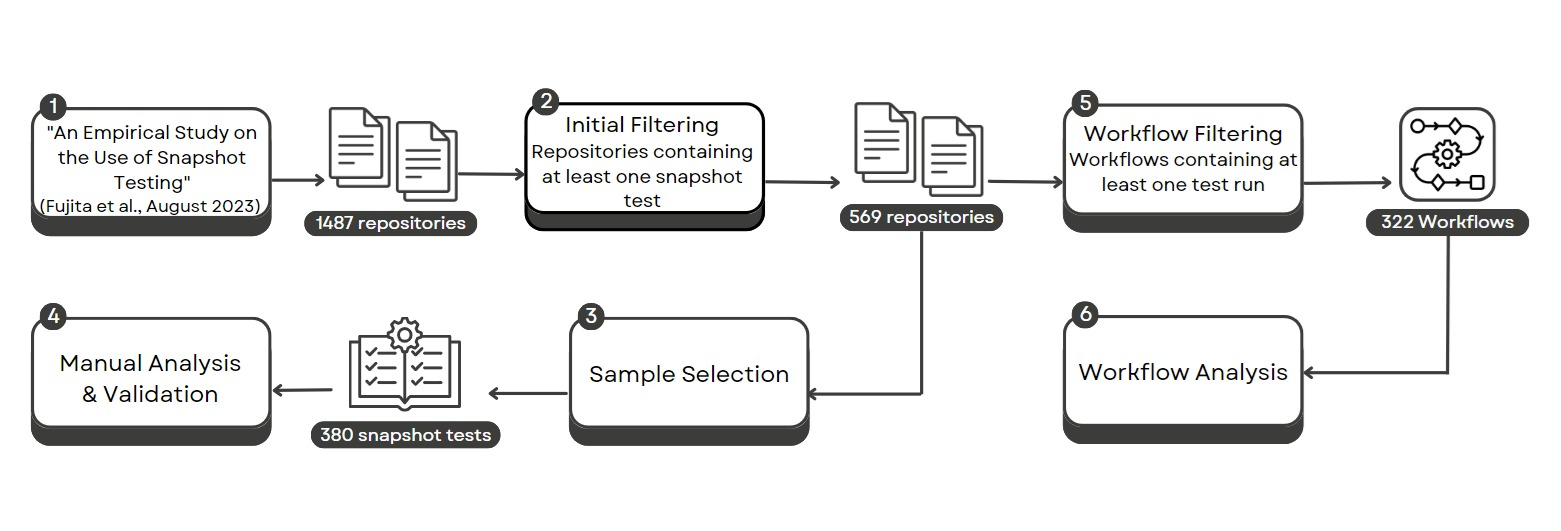
\includegraphics[width=\textwidth]{exemplo/img/study_design_steps.png}
            \caption{Overview of the empirical study steps.}
        \end{figure}

        \begin{enumerate}

        \item\textbf{Replication Package Examination}: We began by examining and reusing a previous study's~\cite{fujita2023empirical} replication package with open-source repositories. This package contained a dataset of 1,487 non-forked GitHub JavaScript and TypeScript projects using Jest, all with more than 1,000 stars. Analyzing its replication package, we were able to identify attributes and metrics such as number of test methods, assertions, and snapshot methods.

        \item\textbf{Initial Filtering}: We filtered the dataset to select only repositories with at least one snapshot test, resulting in a subset of 569 repositories. This subset was then further analyzed to gain insights into the adoption and implementation patterns of snapshot testing with Jest in multiple projects. Additionally, this selection served as a basis for further data collection of continuous integration attributes. 

        To replicate the experiment and validate the metrics for test methods and assertions—including their snapshot counterparts—as originally measured by the dataset authors, we sought to duplicate the study design outlined by the previous study. Initially, all repositories were downloaded at their last commit hash provided in the dataset. Then, we filtered all repositories that contained test files and conducted a detailed examination of the test code focusing on the high-level constructs present in the code, in the form of an  AST (Abstract Syntax Tree). This analysis was done utilizing the \textit{Babel}\footnote{\url{https://babeljs.io/docs/}} tool. With this, the main author achieved the same metrics for all of the 569 repositories, as they were reported from the original dataset authors.

        \item\textbf{Sample Selection}: We extracted all 34,866 matching snapshot test methods across the 569 repositories. Then, we selected a random sample for manual analysis to ensure the results were statistically significant and representative of the overall dataset. To achieve this, the sample size was calculated using a standard statistical method commonly employed in other empirical studies in the software engineering field~\cite{malhotra2016empirical, cruz2019mobile}. This sample size calculation is based on a z-score of 1.96 (for a 95\% confidence level), a margin of error of 0.05, and a population proportion assumption of 0.5, which are typical parameters for findings with a high confidence level. Therefore, our sample is composed of 380 snapshot tests. These were then randomly selected from the original group of 569 repositories, yielding a distribution with 134 different repositories.

        \item\textbf{Manual Analysis}: In this phase, each of the 380 tests underwent a manual analysis conducted by the main author, aiming to identify coding patterns, anomalies, and noteworthy practices associated with snapshot testing.

        \item\textbf{Workflow Filtering}: Using the GitHub API, we leveraged data on repositories with at least one GitHub Actions workflow setup containing at least one test run. With this, we've identified 21,910 runs across 322 unique workflows distributed among 260 repositories.

        \item\textbf{Workflow Analysis}: We looked into how snapshot tests work in a continuous integration environment of GitHub Actions. Specifically, we looked at how often snapshot tests succeeded in Jest-based pipelines to find out if they were valuable in this context and what the best practices were.

        \end{enumerate}
        
    \section{Results}\label{sec:ch4-results}

        \subsection{What are the key characteristics of snapshot tests? (RQ4.1)}

        The manual analysis of the sample revealed many characteristics of snapshot tests. We analyzed the categories of components under tests, behavior under test, format of the snapshots, and their sizes in Lines of Code (LOC).\\

        \subsubsection{Components Under Test}
        %\noindent\textbf{Components Under Test.} 
        
        Table~\ref{tab:ch4-rq1-1} shows the frequency (Freq) of tests in absolute number (abs), and percentage (\%) in relation to our total sample, where we classified them by the most appropriate architecture layer.
          
        \begin{table}[!ht]
            \centering
            \begin{tabular}{p{5cm}S[table-format=2.1]S[table-format=3]}
                \toprule
                \textbf{Type} & {\textbf{Freq (\%)}} & {\textbf{Freq (abs)}} \\
                \midrule
                Frontend   & 47.6\% & 181 \\
                Middleware & 25.8\% & 98  \\
                Backend    & 24.2\% & 92  \\
                Other      & 2.4\%  & 9   \\
                \bottomrule
            \end{tabular}
            \caption{Components under test.}
            \label{tab:ch4-rq1-1}
        \end{table}

        Table~\ref{tab:ch4-rq1-1} describes, in regards to the component under test (CUT), that frontend components were the most frequent target (47.6\%), followed by middleware (25.8\%) and backend (24.2\%) components. A small percentage (2.4\%) fell into the other category, which included components that did not fit neatly into the primary architectural layers.

        These percentages indicate the popularity of snapshot testing for components that are focused on the user interface, which often involves working with HTML or React, likely because of the importance that visual components place on maintaining consistency. Based on the data, snapshot testing seems to have a non-negligible amount of use in middleware and backend code, as it is used to ensure consistency in data transfer subjects. The middleware layer accounted for more than one-fourth of the tests, suggesting a significant use of snapshot testing to verify other client-side functions, but which are not directly related to user interface concerns. The backend layer was tested in almost one-fourth of the cases, reflecting the use of snapshot testing to validate business rules, controllers, repositories, embedded code services, or utility functions, as illustrated in Listing~\ref{lst:bckend-1}.\\ 

        \begin{lstlisting}[language=javascript, caption=Snapshot test in \texttt{amzn/style-dictionary} , label=lst:bckend-1]
        it('import override should match snapshot', () => {
           file.options.import = ["UIKit", "AnotherModule"];
           expect(format(createFormatArgs({dictionary, file, platform: {}}), {},file)).toMatchSnapshot();
        });
        \end{lstlisting} 
        ~\\[-2.0pt]


        \subsubsection{Behavior Under Test}
        %\noindent\textbf{Behavior Under Test.} 
        
        Table~\ref{tab:ch4-rq1-2} presents our classification based on the behavior under test, specifically whether a test method verifies the normal expected behavior of a component or an exceptional one.

        \hspace{1pt}
        \begin{table}[!ht]
        \centering
        \begin{tabular}{p{5cm}S[table-format=2.1]S[table-format=3]}
            \toprule
            \textbf{Behavior} & {\textbf{Freq (\%)}} & {\textbf{Freq (abs)}} \\
            \midrule
            Normal       & 88.7\% & 337 \\
            Exceptional  & 11.3\% & 43  \\
            \bottomrule
        \end{tabular}
        \caption{Behavior under test.}
        \label{tab:ch4-rq1-2}
        \end{table}

        The table shows the majority of snapshot tests (88.7\%) focused on verifying normal or expected behavior. A smaller portion (11.3\%) addressed exceptional behavior, including error handling and edge cases. This suggests that snapshot tests are predominantly used as a first line of defense, similar to smoke tests, to ensure basic functionality and prevent regressions in common use cases, rather than to test for exceptional conditions.

        \subsubsection{Format of Snapshots}
        %\noindent\textbf{Format of Snapshots.} 
        
        Snapshot tests compare the state of a component against a previously stored golden standard. Therefore, we analyzed the format of the stored snapshots. According to the data presented in Table~\ref{tab:snapshot_textual_format}, the snapshots in this sample have a preference for HTML (42.9\%) and JSON (33.2\%), with string snapshots accounting for the remaining (23.9\%). This aligns with the prevalent use of snapshot testing for user interface components, where HTML and JSON are commonly used for data representation and serialization.

        \hspace{1pt}
        \begin{table}[!ht]
            \centering
            \begin{tabular}{p{5cm}S[table-format=2.1]S[table-format=3]}
                \toprule
                \textbf{Format} & {\textbf{Freq (\%)}} & {\textbf{Freq (abs)}} \\
                \midrule
                HTML   & 42.9\% & 163 \\
                JSON   & 33.2\% & 126 \\
                String & 23.9\% & 91  \\
                \bottomrule
            \end{tabular}
            \caption{Snapshot textual format.}
            \label{tab:snapshot_textual_format}
        \end{table}


        \subsubsection{Size}
         %       \noindent\textbf{Size.} 
         
        Another aspect of our characterization in this study was to compute and analyze the distribution of lines of code (LOC) across all tests in our sample. Table~\ref{tab:statistical_summary} summarizes key metrics of this distribution, showing the minimum, first quartile (Q1), second quartile or median (Q2), third quartile (Q3), outlier range, and maximum. As we can see, LOC ranges from a minimum of 3 to a maximum of 306. The quartiles (Q1, Q2, and Q3) are 8, 14, and 26 LOC, respectively. Moreover, tests with 53 or more LOC are classified as outliers.

        \hspace{1pt}
        \begin{table}[!ht]
        \centering
        \begin{tabular}{cccccc}
            \toprule
            \textbf{Min} & \textbf{Q1} & \textbf{Q2} & \textbf{Q3} & \textbf{Outlier} & \textbf{Max} \\
            \midrule
            3 & 8 & 14 & 26 & 53 & 306 \\
            \bottomrule
        \end{tabular}
        \caption{Distribution of snapshot tests size (in LOC).}
        \label{tab:statistical_summary}
        \end{table}

        Since these metrics will be used in the identification of large tests in the following sections (more specifically, research questions 4.2 and 4.3), it is important to clarify how outliers are defined. We used the same outlier calculation as in boxplots. Outliers correspond to data points beyond the third quartile (Q3) plus 1.5 times the Interquartile Range (IQR). For our sample, the third quartile is 26 LOC, and the interquartile range is 18 LOC. Therefore, we considered tests as outliers if they had LOC greater than 53. Specifically, in our sample, twenty-nine tests (7.6\%) were identified as outliers.

        Analysis of the lines of code in each snapshot test indicates that the majority are rather short, with a median size of 14 LOC. This shortness can be a big benefit of snapshot testing because it makes tests easier to write, understand, and keep up to date. However, the presence of large outliers in this distribution suggests that developers should be careful to keep snapshots brief and avoid including inline snapshots that are too big in their tests.

        \subsubsection{Summary of the Characterization}

        Snapshot tests predominantly test front-end components (47.6\%), primarily focus on normal behaviors (88.6\%), and most frequently produce outputs in HTML format (42.8\%). Moreover, they are typically small (median size of 14 LOC).

        \subsection{What are the most common patterns of snapshot tests? (RQ4.2)}

        After the characterization reported in the previous section, we focused on identifying the most common patterns of snapshot tests. Specifically, we identified two main patterns of snapshot tests: Regular and Inline Snapshots. Regular Snapshots store their output in separate files, while Inline Snapshots store their output within the test code itself. Table~\ref{tab:patterns} shows the results of applying this categorization of snapshot tests to our sample. The results indicate that 85\% of the tests follow one of these patterns, confirming they are indeed common patterns.

        \hspace{1pt}
        \begin{table}[!ht]
        \centering
        \begin{tabular}{p{5cm}S[table-format=2.1]S[table-format=3]}
            \toprule
            \textbf{Format} & {\textbf{Freq (\%)}} & {\textbf{Freq (abs)}} \\
            \midrule
            Regular Snapshot & 61.3\% & 233 \\
            Inline Snapshot  & 23.7\% & 90  \\
            Total            & 85.0\% & 323 \\
            \bottomrule
        \end{tabular}
        \caption{Snapshot test patterns.}
        \label{tab:patterns}
        \end{table}

        Understanding these patterns can provide valuable insights for developers, helping them write more effective and maintainable snapshot tests. In this section, we use the term pattern to refer to the anatomy and syntactic structure of such tests. An analogy can be made with unit tests, which usually follow the AAA pattern, an acronym for Arrange, Act, and Assert ~\cite{khorikov2020unit}.
        
        During our analysis of the 380 snapshot tests, we concentrated on identifying recurring structures and practices that could be considered common patterns of snapshot testing. Our goal was to not only document these patterns but also to assess whether they represent best practices for implementing snapshot tests. In the following sections, we present these patterns. The presentation has four key parts: description, structure, example, and exclusion criterion.


        \subsubsection{Regular Snapshots}

        \noindent\textbf{Description:} Following a structure that is similar to the regular Jest example for snapshot tests, the Regular Snapshot pattern we discovered has 233 occurrences (61.3\%), where the output of the component under test is converted to a textual representation and stored in a separate snapshot file with a \texttt{snap} extension.\footnote{\url{https://jestjs.io/docs/snapshot-testing\#snapshot-testing-with-jest}}\\

        \noindent\textbf{Structure:} The structure for this pattern is illustrated in Listing~\ref{lst:regular-snapshot-example}. According to this structure, in a Regular Snapshot, we should convert the CUT into a textual representation and store it in a local variable (line 1). Then, we call the assertion \texttt{toMatchSnapshot()} (line 2).\footnote{\url{https://jestjs.io/docs/expect\#tomatchsnapshotpropertymatchers-hint}}\\

        \begin{lstlisting}[language=javascript, caption= Regular snapshot pattern, label=lst:regular-snapshot-example]
    const component = cut.toRepresentation();
    expect(component).toMatchSnapshot();
        \end{lstlisting} 
        ~\\[-2.0pt]

        \noindent\textbf{Example:} Listing~\ref{lst:regular-snapshot-pratical-example} shows a test method from the \texttt{airbnb/react-sketchapp} repository that follows this pattern.\footnote{\url{https://github.com/airbnb/react-sketchapp/blob/b238e69c6f1e65ec6b1d8a908a91fbd9a8cc43a7/__tests__/jest/components/Image.tsx\#L60}}
        In this example, the developer creates a React component called \texttt{<Image/>} converts it to a representation, and saves it in the local variable \texttt{tree} (line 2). Then, the developer asserts whether this representation matches the snapshot described in a different file (line 3).\\

        \begin{lstlisting}[language=javascript, caption= Regular snapshot test in \texttt{airbnb/react-sketchapp}, label=lst:regular-snapshot-pratical-example]
    it('translates none', () => {
        const tree = renderer.create(<Image source="foo" resizeMode="none" />).toJSON();
        expect(tree).toMatchSnapshot();
    });
        \end{lstlisting}
        ~\\[-2.0pt]

        \noindent\textbf{Exclusion Criterion:} 
        When searching for patterns, we found that some tests following the structure of Listing~\ref{lst:regular-snapshot-example} were quite large. Therefore, they did not meet our criterion that a pattern must represent a good test. Thus, we decided to apply an additional exclusion criterion: a regular snapshot cannot be an outlier in the test size distribution. As discussed in RQ 4.1, we identified 29 outliers in our sample, with sizes ranging from 55 to 304 LOC. Consequently, none of them were classified as regular snapshots, even if they had the structure defined in Listing~\ref{lst:regular-snapshot-example}. Instead, these tests were categorized as unusual cases, which we will discuss in the next research question.

         \subsubsection{Inline Snapshots} 

        \noindent\textbf{Description:} The second most common pattern found was the Inline Snapshot, present in 90 tests (23.7\%). Unlike Regular Snapshots, which store snapshots externally and utilize the regular \texttt{toMatchSnapshot()} assertion, Inline Snapshots uses the \texttt{toMatchInline\-Snapshot(...)} assertion,
        allowing to embed the serialized snapshot directly within the test code as a string literal. Providing a concise way to verify component outputs without managing external files, by only comparing the embed snapshot in the form of a function argument.\footnote{\url{https://www.jestjs.io/docs/snapshot-testing/\#inline-snapshots}}\\

        \noindent\textbf{Structure:} Listing~\ref{lst:pattern-2} illustrates the basic structure of this pattern. First, we save the result from the function under test (\texttt{fut}), which should be part of a component object (line 1). Second, we call the assertion \texttt{toMatchInlineSnapshot(...)} (line 2). The string constant used as the argument of this assertion is used to verify whether the test passes (line 2).\footnote{\url{https://jestjs.io/docs/expect\#tomatchsnapshotpropertymatchers-hint}}\\

        \begin{lstlisting}[language=javascript, caption=Inline snapshot pattern, label=lst:pattern-2]
 const result = component.fut();
 expect(result).toMatchInlineSnapshot(`{state1:value, ...}`);
        \end{lstlisting}

        \noindent\textbf{Example:} Listing~\ref{lst:inline-snapshot-pratical-example} shows a test method from the \texttt{statoscope/statoscope} repository that follows this pattern.\footnote{\url{https://github.com/statoscope/statoscope/blob/9c5b4cef601f8211bd937b0bb2786bc49f133f02/packages/helpers/src/jora/index.spec.ts\#L101-L104}} This test captures the output of a color helper function and uses \texttt{toMatchInline\-Snapshot(...)} with string literals representing the expected color values in HSL format.\\

        \begin{lstlisting}[language=javascript, caption= Inline snapshot test in \texttt{statoscope/statoscope}, label=lst:inline-snapshot-pratical-example]
    test('color', () => {
        expect(helpers.color('foo')).toMatchInlineSnapshot(`"hsl(54, 50%, 85%)"`);
        expect(helpers.color('bar')).toMatchInlineSnapshot(`"hsl(99, 50%, 85%)"`);
    });
        \end{lstlisting}

        \noindent\textbf{Exclusion Criterion:} For Inline Snapshots, we used the same exclusion criterion proposed for regular snapshots, i.e., the test should not be an outlier in terms of size in lines of code. Especially for smaller, self-contained components or pure functions with simple outputs, inline snapshots offer advantages in terms of test readability and ease of management. Due to the fact that the intended output is displayed immediately within the test code, developers are able to directly read and comprehend the snapshot in order to update it whenever it is required. On the other hand, Inline Snapshots can become troublesome if the output expands to an extremely large size. This may result in test files that are bloated and a decrease in readability.

        \subsubsection{Lessons Learned from Snapshot Patterns} 
        
        In the results for this research question, we presented two patterns for snapshot testing with Jest, Regular Snapshots, and Inline Snapshots. Each of these patterns has an individual set of benefits to offer its users. The use of Regular Snapshots allows for a distinct separation between the test logic and the snapshot data, which makes them an great choice for components that are complex and have the capacity to produce huge outputs.
        
        On the other hand, Inline Snapshots are particularly useful for straightforward components or functions that produce small outputs, which provide improved readability and make the management of snapshots less complicated.
        
        The selection of one of these patterns over another is situational, based on the particular circumstances of the project and the test, as well as the features of the component that is being evaluated. However, our investigation indicates that both patterns provided that they are implemented appropriately and succinctly (particularly when making an effort to avoid having a large test method), constitute best practices for snapshot testing. By adhering to these patterns and following the recommended exclusion criteria, developers can make use of the benefits of snapshot testing while also reducing the potential drawbacks, such as concerns with maintainability and fragility.

        \subsection{What are the less-common cases of snapshot tests? Do they constitute test smells? (RQ4.3)}

        Despite the fact that the Regular and Inline Snapshot patterns are the most common ones used for snapshot testing, our manual examination of 380 tests showed certain variations that are less common but nonetheless noteworthy. These uncommon situations, which differ from the regular patterns, provide insights into potential areas for improvement in the techniques and implementation of snapshot testing. We deemed it noteworthy to understand these variances to deepen our knowledge of snapshot testing practices and also to recognize potential test smells that might have an adverse impact on the maintainability of snapshot test code. In this research, we uncovered a number of unusual cases in which developers used snapshot tests (Table~\ref{tab:snapshot_test_unusual_cases}). We would like to emphasize that not all of them are considered test smells, and some may indeed represent good practices.\\

        \hspace{1pt}
        \begin{table}[!ht]
        \centering
        \begin{tabular}{p{5cm}S[table-format=2.1]S[table-format=2]c}
            \toprule
            \textbf{Type} & {\textbf{Freq (\%)}} & {\textbf{Freq (abs)}} & \textbf{Smell} \\
            \midrule
            Large Snapshot Test     & 7.7\% & 29 & Yes \\
            Non-Snapshot Assertions & 5.3\% & 20 & No  \\
            Non-Linear logic        & 1.8\% & 7  & Yes \\
            Error Snapshot          & 0.2\% & 1  & No  \\ \midrule
            Total                   & 15.0\%  & 57 & --  \\
            \bottomrule
        \end{tabular}
        \caption{Snapshot test unusual cases.}
        \label{tab:snapshot_test_unusual_cases}
        \end{table}

        \subsubsection{Large Snapshot Tests} 

        Some snapshot tests (29 occurrences, 7.6\%) have an unusually high number of lines, classifying them as outliers in our sample. For example, the largest test method\footnote{\url{https://github.com/samdenty/gqless/blob/27e289932cf45536c4e91190b96a4c9ce3d95063/packages/cli/test/generate.test.ts\#L566}}  (304 lines) comes from the repository \texttt{samdenty/gqless}. Listing~\ref{lst:large-snapshot-test-example} presents an edited version of this test to illustrate its composition.

        \begin{lstlisting}[language=javascript, caption=Large snapshot test due to an inline snapshot, label=lst:large-snapshot-test-example]
    test('generate works', async () => {
        const { schemaCode } = await generate(server.graphql.schema);

        expect(schemaCode).toMatchInlineSnapshot(`
          "/**
           * GQLESS AUTO-GENERATED CODE: PLEASE DO NOT MODIFY MANUALLY
           */

           import { SchemaUnionsKey } from 'gqless';

           export type Maybe<T> = T | null;
           export type Exact<T extends { [key: string]: unknown }> = {
                [K in keyof T]: T[K];
           };
           ...
        `);
    })
        \end{lstlisting}
        ~\\[-2.0pt]
                  
        In this test, the fixture comprises only one line of code (line 2), while most remaining lines are part of the inline assertion string. Consequently, we consider this implementation a bad smell. As we discussed earlier, inline snapshots are recommended mostly for simpler and smaller outputs. For complex and longer outputs, developers should favor regular snapshots based on external files to avoid cluttering the test method.
            
        \subsubsection{Non-Snapshot Assertions}
            
        Our analysis found twenty tests (5.2\%) that combined snapshot assertions (e.g., \texttt{toMatchSnapshot()}) with other types of assertions, such as \texttt{toBe(...)} or \texttt{toEqual(...)}. This practice, although less frequent, offers a different way to enhance the feedback provided by snapshot tests. For example, Listing~\ref{lst:Non-Snapshot-Assertions-example} shows a test from the \texttt{geist-org/react} repository.\footnote{\url{https://github.com/geist-org/geist-ui/blob/bb575498fed75709e465bee84b2e15f206662cfa/components/button/__tests__/icon.test.tsx\#L19}} In this example, the developer creates a React component and assigns it to \texttt{wrapper} (line 2). Then, the text of a property is stored in a local variable (line 3). The developer uses a \texttt{toMatchSnapshot()} assertion to test the HTML of the component (line 4) and then uses a non-snapshot assertion (\texttt{toBe(0)}) to verify that the text length is zero (line~5).\\
            
            \begin{lstlisting}[language=javascript, caption=  Non-snapshot assertions in \texttt{geist-org/react}, label=lst:Non-Snapshot-Assertions-example]
    it('should work without text', () => {
        const wrapper = mount(<Button iconRight={<Icon/>}/>)
        const text = wrapper.find('.text')
        expect(wrapper.html()).toMatchSnapshot()
        expect(text.length).toBe(0)
    });
            \end{lstlisting}

            On the one hand, using other assertions with this test is redundant, as the snapshot is already able to warn about any change. On the other hand, this assertion provides a detailed and more specific error message in case of failure.
            
            Therefore, combining snapshot and non-snapshot assertions provides more targeted feedback when the test fails. Suppose the snapshot matches but the text length is incorrect. In that case, the developer immediately knows the specific source of the error without needing to examine a potentially large snapshot diff. However, it's important to strike a balance when using Non-Snapshot Assertions alongside snapshots. If overused, they can negate the advantages of snapshot testing by increasing the test's complexity and reducing its conciseness. Developers should consider Non-Snapshot Assertions as complementary checks, providing targeted feedback for specific aspects of the component's output while relying on the snapshot to verify the overall structure. This approach can enhance the diagnostic value of snapshot tests without compromising their main benefits.

            Finally, tests that mix snapshot and non-snapshot assertions are less common, but we do not see them as smells that require refactoring.
            
            \subsubsection{Non-Linear Logic}

            Another test smell occurs when a test lacks a straightforward linear logic. The most common example is the use of conditional statements (e.g., \texttt{if}, \texttt{else}, \texttt{switch} ...) inside a test, as this introduces non-linear logic. This practice can lead to a complex control flow and reduces the clarity of the test's purpose. In our sample, we discovered only seven tests that exhibit this smell (1.8\%).
            As an example, Listing~\ref{lst:Non-Linear-Logic-example} shows an edited test from the \texttt{elastic/kibana} repository.\footnote{\url{https://github.com/elastic/kibana/blob/0645a3ba388f81fc6b43136e64ad53614101e947/src/core/server/saved_objects/version/decode_version.test.ts\#L23}} This test triggers an exception (lines 3-7), whose message is then checked using a \texttt{toMatchInlineSnapshot} (line 8). However, the testing framework offers the assertion \texttt{toThrowErrorMatchingInlineSnapshot()} to handle error messages, which would be more appropriate and easier to use and understand in this specific case.

            \begin{lstlisting}[language=javascript, caption= Non-linear test in \texttt{elastic/kibana}, label=lst:Non-Linear-Logic-example]
    it('throws Boom error if not in base64', () => {
        let error;
        try {
            decodeVersion('[1,4]');
        } catch (err) {
            error = err;
        }
        expect(error.message).toMatchInlineSnapshot('"Invalid version [[1,4]]"');
        expect(Boom.isBoom(error)).toBe(true);
        expect(error.output).toMatchInlineSnapshot(...);
    });
            \end{lstlisting}
            
            The \texttt{try/catch} block presented in this example and other types of conditional checks can introduce branching within the test, making it harder to follow and potentially obscuring the core assertion. While there might be legitimate reasons for using conditional logic in certain testing scenarios, such as handling different edge cases or testing for specific error conditions, developers should generally strive for linear test execution to maximize clarity and maintainability. For this reason, we consider these types of implementations a test smell.

        \subsubsection{Error Snapshots}
        
        Finally, our last case to report is the Error Snapshot, which has only one occurrence in our sample. As previously mentioned, Jest provides the assertion \texttt{toThrow\-ErrorMatchingSnapshot()} to check snapshots in exceptional cases. Listing~\ref{lst:Error-Snapshot-example} shows the single test in our sample that uses this assertion.\footnote{\url{https://github.com/lint-staged/lint-staged/blob/1d39241d236c837fce57cc8bd66a886bd5273c69/test/unit/validateConfig.spec.js\#L63}} In this test, the developer calls the method \texttt{validateConfig} (line 15), expecting it to throw an error, which is checked by the \texttt{toThrowErrorMatchingSnapshot()} assertion.\\
           
        \begin{lstlisting}[language=javascript, caption=  Error snapshot snippet from \texttt{okonet/lint-staged}, label=lst:Error-Snapshot-example]
    it('should throw when detecting deprecated advanced configuration', () => {
        const advancedConfig = {
            chunkSize: 10,
            concurrent: false,
            globOptions: { matchBase: false },
            ignore: ['test.js'],
            linters: { 
                '*.js': ['eslint'] 
            },
            relative: true,
            renderer: 'silent',
            subTaskConcurrency: 10,
        }
        
        expect(() => validateConfig(advancedConfig, configPath, logger)). toThrowErrorMatchingSnapshot()
        expect(logger.printHistory()).toMatchSnapshot()
    });
        \end{lstlisting}
           
        While generally a good practice for testing exceptional cases, the infrequent use of Error Snapshots in our sample is noteworthy. It suggests a potential lack of awareness among developers regarding this specific Jest functionality or perhaps an reliance on traditional \texttt{try/catch} blocks and manual assertions for verifying error messages. Error Snapshots offer a more concise and readable way to test for exceptions than manual assertions and should be considered a best practice for improving the maintainability and clarity of tests involving error handling. Promoting the adoption of Error Snapshots through documentation, examples, and developer training could enhance the overall quality of snapshot testing practices.

        \subsubsection{Lessons learned from less-common cases of Snapshot tests}

         Examining less-common snapshot test cases offers insights into improving snapshot testing techniques. These cases, while sometimes signaling potential test smells such as Large Snapshot Tests and Non-Linear Logic, also serve as opportunities for developers to reflect on and refine their testing practices. By analyzing real-world examples from open-source repositories, developers are exposed to diverse testing trends and challenges that they might not encounter in isolated or proprietary environments. This exposure helps them with their perspective, supporting the adoption of more maintainable methods.

        Together with the previously presented common patterns, the investigation of these less-common cases exposed chances to improve snapshot testing methods by refactoring. Refactoring, for example, assists with symptoms of test smells that fit Large Snapshot Tests' tendency of overwhelming codebases and Non-Linear Logic inclination for cyclomatic complexity. With this in mind, we present our refactoring suggestions in the next section.


        \subsection{What are the snapshot test-specific refactorings? (RQ4.4)}
        
        Our analysis of common patterns and less-common cases of snapshot tests revealed two specific test smells: Large Snapshot Tests and Snapshot Tests with Non-Linear Logic. These smells can hinder the maintainability and readability of tests, making them more prone to errors and harder to update. To address these issues, we propose two novel refactoring techniques tailored specifically for snapshot tests with Jest: \textit{Moving Snapshots to External Files} and \textit{Removing Try-Catch Blocks When Testing for Errors}. These techniques are designed to improve the internal structure of snapshot tests, thus improving their long-term maintainability. These specific refactorings offer practical solutions for developers to address the identified test smells and promote best practices in snapshot testing.
        
        \subsubsection{Move Snapshot to an External File}
        
        This refactoring targets the Large Snapshot Test smell, which occurs when inline snapshots grow excessively large, cluttering the test code and making it harder to read and understand. The core idea behind this refactoring is to move the large inline snapshot from the test code into a separate external file. This reduces the size and complexity of the test method itself and improves the overall organization of the test suite. This refactoring process involves replacing the \texttt{toMatchInlineSnapshot(...)} assertion with \texttt{toMatchSnapshot()}, which instructs Jest to store the snapshot in an external file. For example, consider an inline snapshot to verify the output of a function, such as:
        
        \begin{lstlisting}[language=javascript, caption=Large snapshot test due to an inline snapshot, label=lst:Move-Snapshot-to-an-External-File-example]
    test('generates the correct output', () => {
        const output = generateOutput(inputData);
        expect(output).toMatchInlineSnapshot(`
            Object {
                "id": "123",
                "name": "Test",
                "values": Array [
                  1,
                  2,
                  3,
                  ...
                ]
            }
        `);
    });
                
        \end{lstlisting}
        
        To refactor this test using the Move Snapshot to an External File refactoring method, we should first verify that the test passes. Then, we change the assertion to \texttt{toMatchSnapshot()}, in which Jest will automatically move the snapshot to an external file the next time the test runs. 
        
        The refactored test shown in Listing~\ref{lst:Move-Snapshot-to-an-External-File-2-example} exemplifies the inline snapshot has been moved to an external file as part of changing the assertions. The test method with reduced lines of code is more concise. This refactoring improves the readability of the test and makes it easier to manage updates to the expected output, as changes are now reflected in a separate snapshot file rather than within the test code itself.

        \begin{lstlisting}[language=javascript, caption=  Snapshot test after moving snapshot to an external file, label=lst:Move-Snapshot-to-an-External-File-2-example]
    test('generates the correct output', () => {
        const output = generateOutput(inputData);
        expect(output).toMatchSnapshot();
    });
                
        \end{lstlisting}       
        
        \subsubsection{Removing Try-Catch when Testing for Errors}
        
         The second refactoring technique addresses the Non-Linear Logic test smell, which arises when snapshot tests incorporate conditional logic (e.g., \texttt{try/catch} blocks) to handle potential errors or exceptions. This can make tests harder to understand and maintain due to the introduction of branching and nested code blocks. Our proposed refactoring removes the \texttt{try/catch} block and replaces it with Jest's specialized assertion \texttt{toThrowErrorMatchingInlineSnapshot(...)}. This assertion allows developers to directly capture and verify the error message thrown by the component under test without the need for logic branching. This simplifies the test structure, making it more linear and easier to comprehend. 
        
        For example, Listing~\ref{lst:Removing-Try-Cath-example} presents a test that verifies if an exception is thrown with a specific error message using an inline snapshot. In lines 3-7, the test fixture catches any errors thrown by the \texttt{validateInput('')} function, and assigns it to a variable. In line~8, the error message is compared against an inline snapshot to confirm it matches the expected error message: ``\textit{Invalid input: Input cannot be empty.}"
        
        \begin{lstlisting}[language=javascript, caption=  Snapshot test with non-linear logic, label=lst:Removing-Try-Cath-example]
    it('throws an error when input is invalid', () => {
        let error;
        try {
             validateInput('');
        } catch (err) {
            error = err;
        }
        expect(error.message).toMatchInlineSnapshot("Invalid input");
    });         
        \end{lstlisting}
        
        Listing~\ref{lst:Removing-Try-Cath-2-example} shows this refactoring applied to the previous example.
        
        \begin{lstlisting}[language=javascript, caption=Snapshot test after applying removing try-catch when testing
 for errors, label=lst:Removing-Try-Cath-2-example]
    it('throws an error when input is invalid', () => {
        expect(() => validateInput(''))
        .toThrowErrorMatchingInlineSnapshot("Invalid input");
    });
                
        \end{lstlisting}

        This refactored code is generally preferred for its conciseness and readability when specifically testing for error conditions, as it reduces unnecessary code and improves clarity.

        \subsubsection{Summary of Snapshot Test Refactorings} 
        
        The two refactoring methods presented in this section, \textit{Moving Snapshots to External Files} and \textit{Removing Try-Catch When Testing for Errors}, address specific test smells related to snapshot size and control flow. They are designed to improve the readability, maintainability, and diagnostic capabilities of snapshot tests, promoting best practices and enhancing the overall effectiveness of snapshot testing as a technique for ensuring software quality. Table~\ref{tab:snapshot_test_smells_refactorings} summarizes the two identified snapshot test smells and the proposed refactorings presented.

        \hspace{1pt}
        \begin{table}[!ht]
        \centering
        \begin{tabular}{p{3cm}p{7cm}p{4cm}}
            \toprule
            \textbf{Test Smell} & \textbf{Description} & \textbf{Refactoring Technique} \\
            \midrule
            Large Snapshot Test & Inline snapshots become excessively large, cluttering test code and reducing readability. & Move Snapshot to an External File \\
            \midrule
            Snapshot Test with Non-Linear Logic & Conditional logic (try/catch) within tests introduce branching and reduce clarity, hindering understanding and maintenance. & Removing Try-Catch when Testing for Errors \\
            \bottomrule
        \end{tabular}
        \caption{Snapshot test smells and refactorings.}
        \label{tab:snapshot_test_smells_refactorings}
        \end{table}

        \subsection{Should we use snapshot tests in CI pipelines? If so, what are the best practices? (RQ4.5)}
        
        The purpose of this section is to explore the usage of snapshot tests inside Continuous Integration and Continuous Delivery (CI/CD) pipelines focusing on GitHub Actions. Previous sections explored the static properties and typical coding patterns of snapshot tests, but this analysis offers a more dynamic approach.
        
        Our aim is to verify whether snapshot tests should be included into continuous integration and continuous delivery pipelines and, if so, to identify best practices for their effective use and maintenance in this context. Snapshot tests with Jest challenge integration into these pipelines due to the nature of a software project that constantly updates the snapshot reference. Failing on these updates allows for false positives, demanding more effort and time from the developers. On the other hand, relying too much on automatic snapshot updates can mask regressions and lead to decreasing confidence in the test suite.

        For this research question, we returned to the 569 repositories with at least one snapshot test from our original dataset. We found that 388 repositories (73\%) had GitHub Actions workflows configured. We examined the specific configuration of these workflows to determine how many of them have tests executed with Jest. We concluded that 363 repositories (63\%) run Jest tests in their workflows, indicating regular usage of continuous testing on pushes and pull requests. After that, we verified which repositories had open logs for their workflow runs. We found 260 repositories (45\%) with at least one workflow from which we could retrieve run data. From those repositories, we collected 21,910 test runs across 322 different workflows. Finally, we used custom scripts to determine whether the runs finished successfully or not, and then calculated the average success/failure rate for each workflow.

        To collect and analyze this data, we implemented extraction scripts that utilized the GitHub API ~\footnote{\url{https://docs.github.com/pt/rest?apiVersion=2022-11-28}} to retrieve workflow execution details. Specifically, we queried the \texttt{repos/owner/repo/actions/workflows} endpoint to identify repositories with GitHub Actions workflows, followed by \texttt{repos/owner/repo/actions/runs} to collect metadata on workflow executions. Additionally, we accessed the \texttt{repos/owner/repo/actions/runs/\\id/logs} endpoint to retrieve detailed logs for test execution results. These logs were further analyzed using regular expressions (regex) to identify failures explicitly related to snapshot testing. The regex patterns allowed us to detect failure messages indicating snapshot mismatches, ensuring reliablility. By automating this process, we were able to extract trends and evaluate the extent to which snapshot test fragility impacts CI pipelines.
        
        In our analysis of the 21,910 workflow runs across 322 distinct workflows we found that 6,402 runs (29\%) resulted in failures. Out of these failures, using custom scripts to analyze open logs and determine the reasons that led to the failure of each specific run, only 1,129 (5\%) were directly caused by failed snapshot tests. We found this relatively low percentage surprising since fragility is the main drawback reported for snapshot tests in our Grey Literature Review (Section~\ref{sec:ch3-drawbacks}).

        Figure~\ref{fig:empirical-histogram} displays a histogram of average successful run percentages, with the x-axis representing the average percentage of successful runs and the y-axis showing the number of workflow runs per percentage interval.

            \begin{figure}[h]
                \centering
                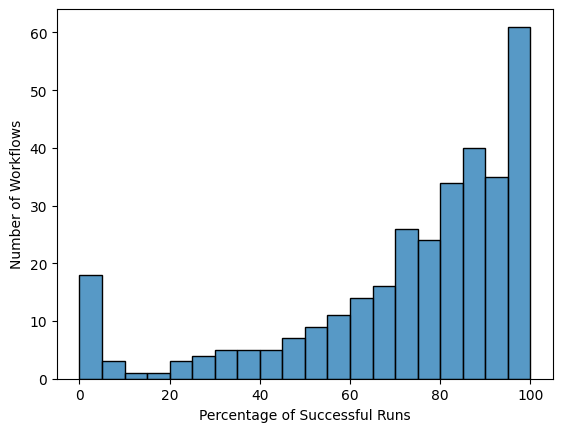
\includegraphics[scale=0.85]{exemplo/img/histogram.png}
                \caption{Histogram of successful run percentages}
                \label{fig:empirical-histogram}
            \end{figure}

        This distribution suggests a skew towards higher success rates, with the majority of workflows achieving a success rate of 80\% or greater, which indicates a notable presence of automated processes within these projects, reflecting a trend towards incorporating snapshot testing in CI/CD. In order to verify this trend, we provide violin and box plots in Figures~\ref{fig:empirical-violin-plot} and~\ref{fig:empirical-box-plot}, as these visualizations provide more informative and detailed comparisons between the ranges present in this distribution, especially across higher success categories as both visualizations smooth out variations and highlights trends.

            \begin{figure}[h]
                \centering
                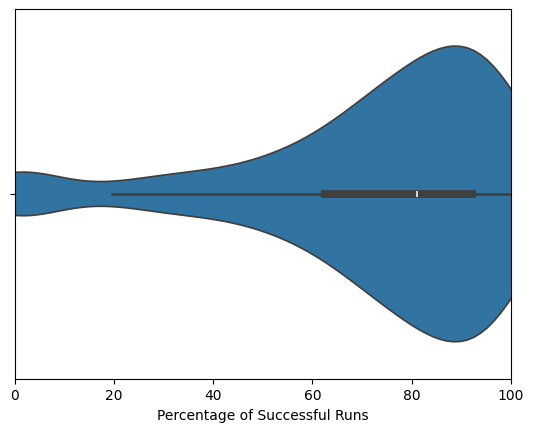
\includegraphics[scale=0.8]{exemplo/img/violin-plot.png}
                \caption{Violin plot of successful run percentages}
                \label{fig:empirical-violin-plot}
            \end{figure}

            \begin{figure}[h]
                \centering
                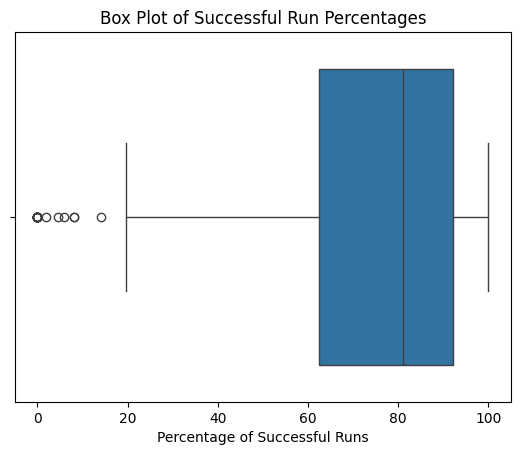
\includegraphics[scale=0.8]{exemplo/img/box-plot.png}
                \caption{Box plot of successful run percentages}
                \label{fig:empirical-box-plot}
            \end{figure}

       Figure~\ref{fig:empirical-violin-plot} shows a concentration of successful runs in the highest success rate range, particularly from 60\% to 100\%. This clustering towards the upper quartiles suggests that most workflows achieve high success rates, implying automated testing setups and effective integration of snapshot testing in continuous integration (CI) pipelines.
        
        Figure~\ref{fig:empirical-box-plot} provides a box plot visualization of the distribution of success rates across the 322 CI workflows analyzed. In this visualization, we can see that the data points beyond the whiskers (considered outliers), range from 0\% to 20\% of successful runs, indicating that workflows with the average success rate below 20\% are very rare.        

        \subsubsection{Best practices of Snapshot in CI/CD}
            
        During our analysis of workflows, we cataloged two important best practices when using snapshot tests in continuous integration environments. Both best practices are associated with Jest and its Command Line Interface (CLI), and can be useful for reducing some issues related to snapshot testing with it.
        
        \begin{enumerate}
            \item \textbf{Use the \texttt{--ci} flag}: The \texttt{--ci} flag in Jest is designed specifically for CI environments. It optimizes test execution and enforces stricter rules for snapshot updates, preventing unintended changes from being automatically updated and saved in newer runs. Newer versions of Jest automatically detect CI environments based on commonly used environment variables, but explicit use of the \texttt{--ci} flag is recommended for clarity and to ensure consistent behavior across different CI systems, which is particularly useful to standardize project configurations.
            \item \textbf{Avoid automatically updating snapshots in CI}: Due to the automated processes found in CI workflows, snapshot updates should not occur automatically within the CI environment. This includes avoiding the \texttt{--updateSnapshot} flag, as unintended changes could be inadvertently saved to the snapshot files, potentially masking regressions. Suggesting that all snapshot updates should be done by the developers running the test locally, following a careful review of the changes in a controlled environment, outside CI.
        \end{enumerate}

        \subsubsection{Lessons learned from Snapshot Testing in CI/CD}
        
        The relatively low failure rate of snapshot tests in CI may indicate that developers are recurrently managing snapshots, which indicates good testing practices overall, minimizing the fragility of the snapshots. Another interesting finding suggests that tests can be effectively integrated into CI pipelines as they skew towards high success rates.
        
        However, this adoption should take into account key points highlighted by the appropriate best practices presented. The identified best practices, using the \texttt{--ci} flag and avoiding automatic snapshot updates in CI, further reinforce the importance of careful snapshot management in automated testing environments. By using the Jest \texttt{--ci} flag and avoiding updating snapshots in CI (e.g. using the \texttt{--update-snapshot} flag), developers can maintain a high quality in their development processes while ensuring automated testing has no overhead on CI circumstances.
        
        \section{Discussion}\label{sec:ch4-discussion}
        
        The patterns identified are specific to the Jest snapshot testing framework. They may not directly apply to other platforms or testing tools, as these may define and implement snapshot testing differently. This specificity highlights the importance of understanding the distinct features and capabilities of the tools employed in software testing. The classification of patterns is based on the functions provided by Jest, reflecting both the framework’s inherent capabilities and its limitations. This classification helps elucidate how different components and functionalities are tested through snapshots, offering a practical resource for developers and practitioners.

        Our findings indicate that snapshot test failures constitute a relatively small percentage (5\%) of overall test failures in Continuous Integration workflows. In our grey literature review, specifically in Section~\ref{sec:ch3-drawbacks} regarding the drawbacks of snapshot testing (RQ3.2), we reported snapshot tests to be fragile, and therefore, we had expected a greater number of CI failures due to snapshot testing. Based on our experience and analysis of snapshot testing, we have formulated two possible explanations for the low failure rate: (1) developers are following a mature software development process which produces fewer snapshot inconsistencies and consequently fewer failures; or (2) developers are resolving snapshot failures locally before pushing code to the CI server. Investigating this would require surveying developers, which is outside the scope of this research, but we consider it an interesting line for future work.

        A notable contradiction emerges when comparing the results of RQ4.1 and RQ3.4, particularly in the backend category. While the results of RQ3.4 suggests that snapshot testing is predominantly associated with frontend components, the results of RQ4.1 reveals a substantial increase in its usage in backend applications. This disparity suggests that the perception of snapshot testing in the industry remains largely focused on the frontend, while some of the actual development practices show a growing adoption of this technique for backend testing, being leveraged as a form of API testing, as service integrations are captured and compared across test runs.

        In conclusion, this empirical research on snapshot testing practices offers valuable insights into the adoption and practical use of this technique, particularly within Jest-based testing environments. By analyzing a substantial dataset of open-source repositories and examining the behavior of snapshot tests in continuous integration pipelines, we identified both common patterns and specific challenges, such as test smells and refactoring suggestions. Our findings underscore the importance of carefully managing snapshot tests to maintain their effectiveness, particularly in large-scale projects. The results of this study not only contribute to the existing body of knowledge on software testing practices but also provide actionable guidance for developers looking to improve the reliability and maintainability of their snapshot test suites. These final reflections highlight the significance of this work as a foundation for future research on extending and refining snapshot testing methodologies.
         
        \section{Threats to Validity}\label{sec:ch4-threats}

        \noindent \textbf{External Validity.} The population for our analysis came from an available dataset composed of public GitHub repositories using Jest. Therefore, the population suffers from the same threats to validity as reported by the dataset original authors~\cite{fujita2023empirical}. Namely, this population may not represent private, and closed-source applications. It may also not represent other testing frameworks or programming languages.
        Moreover, we used random sampling to select test methods for our manual analysis. Since random sample is unbiased, there is relevant evidence for external validity and the generalization of our findings based on the population.
        In our workflow analysis for continuous integration, we automatically evaluated only workflows with open logs, leaving others with closed or private logs unstudied, which could affect the generalization of failed runs caused by snapshot testing.\\
        
        \noindent \textbf{Internal Validity.} Sampling can introduce selection bias to any experiment. However, random sampling reduces selection bias by giving every test in our population an equal chance to be included in the analysis.
        Moreover, the analysis of snapshot tests in our sample could be conducted in automated form, however, we did not have a profound understanding of the Babel tool, making it difficult to automatically match expected Abstract Syntax Trees. In order to mitigate this issue, the analysis was made based on a manual classification for increased accuracy.
        In the workflow analysis for CI, we did not use sampling. Instead, we used a script to automate the process and analyze all run data we had acquired.\\
        
        \noindent \textbf{Construct Validity.} Our reported results are based on a manual classification performed by a single person. Therefore, they might be subjected to mistakes or biased interpretations. Since we opted to analyze objective properties of tests that were expressed in the source code, we believe this bias to be minimal.
        
        \section{Final Remarks}\label{sec:ch4-final-remarks}

        This chapter presented an empirical study investigating snapshot testing practices in real-world software development projects. By analyzing a diverse dataset of snapshot tests and CI workflows, this study provides valuable insights for both practitioners and researchers, furthering our understanding of this relatively new testing technique. We will recap some important discoveries made in this chapter. The concise key points of this empirical study aimed to answer five research questions about snapshot testing. The study employed a mixed-methods approach, combining qualitative analysis of 380 snapshot tests with quantitative analysis of 21,910 CI runs from 322 workflows in 260 open-source repositories.

        In the context of open-source collaborative projects within the software development community, this empirical study offered useful insights into the adoption and implementation of snapshot testing with Jest, as well as the practical applications of this testing method. Through a rigorous examination of over 569 repositories and a carefully selected sample of 380 snapshot tests, we explored important characteristics of snapshot tests, identifying the primary types of components tested and highlighting snapshot testing’s prevalence in frontend components. Additionally, our findings on common and less-common patterns provided insight into structured and atypical usage patterns, such as regular and inline snapshots. Then, the study documented refactoring techniques that optimize test design by managing snapshot size and improving maintainability, offering developers actionable strategies for enhancing snapshot test quality.

        This research proposed two new refactoring methods for snapshot tests — Moving Snapshots to External Files and Removing Try-Catch Blocks when testing for Errors — which aim to address these smells by relocating snapshots and improving code readability and structure and control flow in the tests. This contribution is particularly valuable for developers seeking practical guidance to enhance snapshot testing quality and maintainability within their test suites and to avoid test smells in the long term, minimizing the likelihood of error and improving the quality of testing results, making them more effective when used. It provides concrete, actionable steps to improve test code, making tests easier to write, easier to read, and easier to maintain, ultimately enhancing the overall testing practice.
        
        In regards to Continuous Integration pipelines, we uncovered that the integration of snapshot tests is valuable, as the majority of pipelines tend to have a success rate of over 80\%. We also identified strategies for effective integration, including
        best practices in favor of using environment flags (\texttt{--ci}) and avoiding the automatic update of snapshots, as developers should be the ones that are resolving snapshot failures locally before pushing code to CI servers, to prevent masking potential regressions.

     \chapter{Conclusion}
     
		\section{Overview}
  
        In this master dissertation, two studies were conducted to investigate snapshot testing from different perspectives. The first study employed a grey literature review to analyze 50 documents to explore the practical benefits, drawbacks, and best practices of snapshot testing, gathering information from experienced practitioners and industry sources. The second study followed an empirical approach, analyzing 569 open-source repositories with snapshot tests involving a manual inspection of a random sample of 380 snapshot tests, examining characteristics such as coding patterns, unusual cases, and the use of snapshot tests in continuous integration workflows. Together, we believe these two studies provide a comprehensive view of the current state of snapshot testing with Jest, filling the gap for a later more in-depth exploration of this software testing technique.

        \section{Bridging Perceptions and Practices}

        The results of our study in Section~\ref{sec:ch3-results} provides insights into developers perceptions of snapshot testing based on grey literature, while our results in Section~\ref{sec:ch4-results} empirically examines how snapshot testing is beign implemented in open-source projects. By connecting the research questions from both studies, we can analyze whether developers reported benefits, challenges, and best practices aligned with real-world usage.

        First, the benefits identified in RQ3.1—such as ease of implementation, regression detection, and improved test automation—are reflected in RQ4.1, where we analyze key characteristics of snapshot tests, including the components being tested and how they contribute to software quality.
        
        Similarly, the drawbacks reported in RQ3.2—such as test fragility, excessive maintenance overhead, and lack of meaningful assertions—can be observed in practice through the test smells identified in RQ4.3. Issues like large snapshots, non-linear logic, and excessive reliance on inline snapshots reinforce the concerns raised by practitioners in the grey literature.
        
        To address these challenges, RQ3.3 outlined best practices, including keeping snapshots small, reviewing snapshots carefully, and integrating them with code reviews. These recommendations align with the refactoring strategies discussed in RQ4.4, which propose concrete techniques such as moving large snapshots to external files and removing unnecessary try-catch blocks to improve maintainability.
        
        Lastly, RQ3.4 explores which architectural components are commonly tested using snapshot testing, particularly frontend UI components. This aligns with RQ4.1, where we empirically examined the components under test and confirmed whether snapshot testing is predominantly applied to UI elements or extends to other areas such as API responses and configuration files. Additionally, while snapshot testing is primarily associated with frontend development, RQ4.1 also highlighted its increase in usage for backend services, such as testing serialized data structures, API endpoints, and configuration artifacts, highlighting its broader potential beyond UI validation.
        
        By linking developers perceptions with empirical findings, we bridge the gap between expectations and actual usage, providing a comprehensive perspective on the role of snapshot testing in software development.

		\section{Contributions}
        
        \noindent This master dissertation contributes to the following aspects:
        \begin{itemize}
          \item We discovered that most developers relate to snapshot testing by using Jest as their testing framework for it, especially for the frontend part of applications.
          \item We investigated snapshot testing limitations, shedding light on potential areas for methodological improvement.
          \item We proposed two refactoring operations for snapshot tests, enabling cleaner and more manageable test code.
          \item We offered empirical data on common snapshot test patterns, providing references for software testing standards.
          \item We explored the role of snapshot tests in continuous integration, uncovering their viability when best practices are employed.
          \item We outlined a framework for assessing snapshot testing benefits, facilitating deeper understanding for researchers and practitioners.
        \end{itemize}
        
        \section{Future Work}
        
        In this dissertation, we conducted a grey literature review and an empirical study on snapshot testing with Jest. Possible extensions of this work include: 

        \begin{itemize}
          \item \textbf{Generalization.} Our study focused on snapshot testing with Jest. In this way, as future work, we suggest investigating the adoption of this technique in different programming languages and testing frameworks.
          \item \textbf{Impacts on code coverage.} Snapshot testing is famous for being flexible in its format of snapshot, which can reduce the number of assertions for a test. Therefore, a suggestion for future work is to examine how snapshot tests contribute to or overlap with other forms of testing in the context of code coverage across different project components.
          \item \textbf{Developer Surveys.} We encourage in future works conducting interviews or surveys with developers who regularly use snapshot testing as it could offer additional insights into its practical advantages and challenges.
          \item \textbf{First Snapshot.} The initial snapshot in a series of  tests is important to study as it sets the standard for all following snapshots. Investigations in future work on how these can be properly established can yield interesting results as it reduces the number of updates required for the test to pass.
          \item \textbf{Overlap (or underlap) of snapshot documents}: Future work on 
          grey literature reviews could investigate how snapshot documents relate to each of the different research questions (RQs), possibly using Venn diagrams to illustrate overlaps and gaps in coverage.
          \item \textbf{Historical analysis of snapshot versions}: Inspired by the work of Fujita et al., a longitudinal study could be conducted to analyze the evolution of snapshots over time, identifying trends in modifications and stability.
          \item \textbf{Impact on team productivity}: An empirical study could evaluate the effects of snapshot testing adoption on the productivity of development teams, measuring key performance indicators before and after implementation.
          \item \textbf{Evaluating snapshot tests for edge cases}: A study could revisit the original intent and behavior of snapshot tests in capturing edge cases, determining whether they effectively cover exceptional scenarios or if alternative testing strategies are preferable.
          %\item \textbf{Characterization of snapshot changes}: Future work could analyze the nature of modifications in snapshot tests—whether changes primarily stem from updated values or structural alterations in components. If changes are mostly value-based, it would raise the question of why snapshot testing is preferred over unit testing.
          \item \textbf{When (not) to use snapshot tests}: Further research could explore in which contexts snapshot testing is beneficial or problematic, such as in legacy systems, where frequent updates might be disruptive.
          \item \textbf{Optimizing snapshot tests}: Investigating methods to improve snapshot testing efficiency, such as “shallow” rendering techniques or handling non-deterministic data, could enhance their reliability and usability in CI/CD pipelines.
          
        \end{itemize}
        
		%% Referências
		\renewcommand\bibname{References} %% Trabalhos em inglês
		\bibliographystyle{plain}
		\bibliography{referencias}
		
\end{document}